\chapter{Revisão Bibliográfica}

A pesquisa bilbliográfica deste trabalho é delineada pelo estudo de sistemas
multicorpos, que faz uma revisão da modelagem cinemática e dinâmica desses
sistemas; a análise dinâmica de estruturas, que busca métodos para obter a
matriz de rigidez e amortecimento da base; pesquisa sobre sistemas robóticos
compostos por elementos flexíveis; e por fim tarefas robóticas de precisão
\textit{in situ}.


% -.~.-.~.-.~.-.~.-.~.-.~.-.~.-.~.-.~.-.~.-.~.-
\section{Dinâmica de Sistemas Multicorpos}

A dinâmica de sistemas multicorpos (MBS) é baseada na mecânica clássica. Esses
sistemas são definidos por um ou mais corpos, imperfeitamente conectados, pela
possibilidade de movimento relativo entre eles. A conexão imperfeita de 2 ou
mais corpos rígidos que forma o sistema multicorpo é denominado par cinemático,
ou junta~\cite{de2012kinematic}. Dinâmica multicorpos pode ser entendida como o
estudo de sistemas de vários corpos sujeitos a forças e interações devido a
diferentes tipos de juntas que os conectam e restringem seu
movimento~\cite{flores2008kinematics}, como ilustrado esquematicamente na
Figura~\ref{fig::mbs_diagram}.

\begin{figure}[h]
	\centering 
 	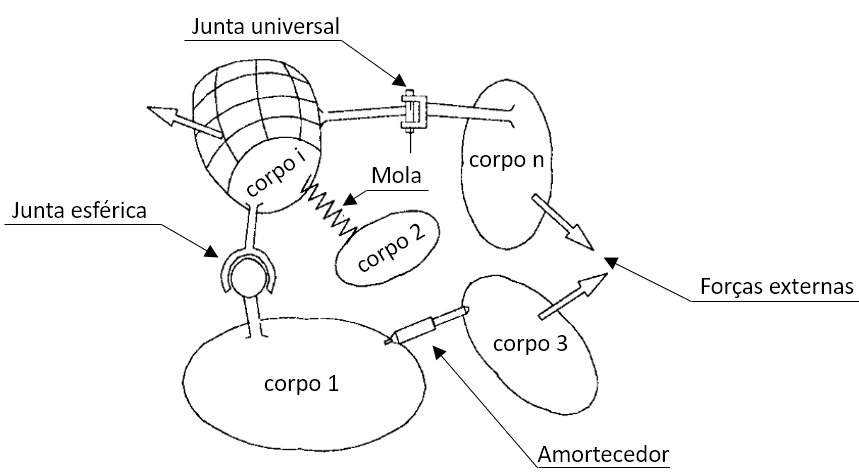
\includegraphics[width=0.75\textwidth]{figs/mbs_diagram}
 	\caption[Representação de um sistema MBS]{Representação de um sistema MBS
 	\\Fonte: adaptado de \cite{neto2003stabilization}}
 	\label{fig::mbs_diagram}
\end{figure}

A mecânica clássica dos sistemas de corpos rígidos e suas aplicações foram
marcadas por fortes restrições na complexidade dos modelos até a década de 1960.
Entretanto, a necessidade de modelar sistemas mais complexos, como satélites e
veículos espaciais, assim como a rápida evolução dos computadores na época,
abriram caminhos para aplicações mais avançadas de sistemas
multicorpos~\cite{schiehlen1997multibody}.

Hoje, muitos programas estão disponíveis para a modelagem e simulação de
sistemas MBS, e possuem interface gráfica e ferramentas para modelagem ou
importação de corpos CAD e elementos padronizados de conectores, como juntas de
de vários tipos, molas e amortecedores. Para citar alguns:
%
\begin{enumerate*}[label=\emph{\roman*})]
	\item MSC ADAMS;
	\item Universal Mechanism;
	\item MapleSim.
\end{enumerate*}
%

No entanto, para ter maior controle da modelagem matemática, dos métodos e das
simplificações e tratamento e pós-processamento dos resultados, este trabalho
não fez uso de um programa comercial dedicado. Para isso, derivou-se toda a
cinemática, dinâmica e equações de movimento dos sistemas simbolicamente, no
Sophia-Maple. Isto permite que o método seja livre de restrições impostas pelas
capacidades destes programas, e torna explícita a metodologia proposta e
permitindo repeti-la e verifica-la em qualquer outra plataforma.

Os fundamentos da cinemática e da dinâmica, tratados a seguir, são reunidos de
livros-texto de referência nas disciplinas de Dinâmica de Corpos Rígidos
\cite{tenenbaum2006fundamentals} e \cite{kane1985dynamics}, Sistemas Multicorpos
\cite{shabana2013dynamics} e Robótica \cite{sciavicco2012modelling} e
\cite{spong2006robot}. Esses autores guiam os conceitos básicos apresentados
nesta seção para modelagem matemática dos sistemas multicorpos.


\subsection{Cinemática}\label{sec::cinematica}

Na análise cinemática de sistemas multicorpos, apenas os aspectos geométricos
são estudados para descrever as posições, velocidades e acelerações dos corpos.
As forças e momentos que causam o movimento do sistema são considerados na
análise dinâmica.

\subsubsection{Sistemas de Coordenadas}

Um corpo rígido é completamente descrito por sua posição e orientação com
respeito a um sistema de coordenadas (SC). Um sistema de coordenadas é um
conjunto de eixos ortogonais que se inteceptam em um ponto, denominado origem.

Geralmente, em sistemas multicorpos, 2 tipos de SC são utilizados. O primeiro é
fixo no tempo e representa uma referência para todos os corpos, denominado
sistema de referência \emph{global} ou \emph{inercial}. O segundo tipo é
solidário a cada componente do sistema, representando um SC \emph{local}, que
translada e gira com o corpo.

A Figura~\ref{fig::sist_refs} apresenta um corpo B, seu referencial local SC-B e
um referncial inercial SC-R, que descrevem o mesmo ponto $p$ em B, por 2 vetores
diferentes.

\begin{figure}[h]
	\centering 
 	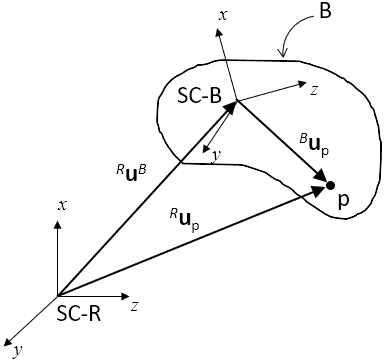
\includegraphics[width=0.45\textwidth]{figs/sist_refs}
 	\caption{Sistemas de referência global e local}
 	\label{fig::sist_refs}
\end{figure}

Os vetores que descrevem a posição do ponto $p$ em cada referencial podem ser
definidos com 3 coordenadas:
%
\begin{align}
	^{R}\textrm{\textbf{u}}^{p} = [r1, r2, r3]^{R} \\
	^{B}\textrm{\textbf{u}}^{p} = [b1, b2, b3]^{B}
\end{align}
%
Note-se que $^{R}\textrm{\textbf{u}}^{p}$ também pode ser escrito como a soma de
2 vetores:
%
\begin{equation}
	^{R}\textrm{\textbf{u}}^{p} = {}^{R}\textrm{\textbf{u}}^{B} + 
	{}^{B}\textrm{\textbf{u}}^{p}
\end{equation}
%

Logo, qualquer ponto no do corpo B pode ser descrito como uma soma da posição do
referencial do corpo, com respeito ao referencial global e o vetor posição do
ponto com respeito ao refencial local.


\subsubsection{Coordenadas generalizadas}

A configuração de um sistemas multicorpos é identificada por um conjunto de
variáveis chamadas \emph{coordenadas generalizadas}, que definem completamente a
posição e orientação de cada corpo no sistema.

Então, um corpo rígido no espaço pode ser descrito usando 6 coordenadas
independentes, 3 para posição da origem do corpo e 3 para orientação do corpo
com respeito ao referencial inercial. Estes parâmetros serão função das
coordenadas generalizadas.

As coordenadas generalizadas são usualmente simbolizadas pela letra
$q$, e numeradas de $1$ a $n$. Podem ser denotadas pelo seguinte vetor:
%
\begin{equation}
	\mathbf{q} = [q1, q2, q3,\ldots, qn]
\end{equation}
%
A variação das coordenadas generalizadas, ou seja, sua derivada no tempo, é
usualmente representada pela letra $u$. Logo:
%
\begin{equation}
	\frac{\mathrm{d} \mathbf{q}}{\mathrm{d} t} = \left[ \frac{\mathrm{d}
q1}{\mathrm{d} t}, ..., \frac{\mathrm{d} qn}{\mathrm{d} t}\right] \rightarrow  \mathbf{u} = [u1,...,un]
\end{equation}
%



% A escolha dos SC's impacta substancialmente no tamanho das equações
% cinemáticas que descrevem os movimentos dos corpos. Uma escolha perspicaz do conjunto de
% SC's utilizado é importante para a eficiência do código e do cálculo
% computacional.

\subsubsection{Matrizes de Rotação}

As matrizes de rotação definem a orientação relativa entre 2 sistemas de
coordenadas. As matrizes que representam as rotações básicas em torno
dos eixos $x, y$ e $z$ de um sistema de coordenadas cartesiano são: 
%
\begin{equation}
	R_{x,\theta} = 
\begin{pmatrix}
1 &0  &0 \\ 
0 &\cos(\theta)  &-\sin(\theta) \\ 
0 &\sin(\theta)  &\cos(\theta) 
\end{pmatrix}
\end{equation}
%
\begin{equation}
R_{y,\theta} = 
\begin{pmatrix}
\cos(\theta) &0  &\sin(\theta) \\ 
0 &1  &0 \\ 
-\sin(\theta) &0  &\cos(\theta) 
\end{pmatrix}
\end{equation}
%
\begin{equation}
R_{z,\theta} = 
\begin{pmatrix}
\cos(\theta) &-\sin(\theta)  &0 \\ 
\sin(\theta) &\cos(\theta)  &0 \\ 
0 &0  &1
\end{pmatrix}
\end{equation}
%

Uma matriz rotação geral $R$, pode ser definida pela sequência ilimitada de
quaisquer rotações básicas. Por exemplo:
%
\begin{equation}
	R_{ZYZ} = R_{z,\phi} \cdot R_{y,\theta} \cdot R_{z,\psi}
\end{equation}
%
Esta em especial representa um método comum para para especificar a matriz de
rotação que orienta um corpo em função 3 quantidades independentes $\phi,
\theta, \psi$, denominado \emph{Ângulos de Euler}, tal que de 3 rotações, não
ocorram 2 rotações sucessivas em torno do mesmo eixo.
Outros métodos comuns para especificar uma matriz de rotação são ângulos
\textit{Roll-Pitch-Yaw}, Quaternions~\cite{sciavicco2012modelling} e ângulos de
Bryan~\cite{wittenburg2013dynamics}.

Também é possível uma representação exponencial da matriz de rotação. É
demonstrado em~\cite{murray1994mathematical}, utilizando o método dos parâmetros
de Rodrigues, como representar a rotação $R \in \mathbb{R}^{3\times3}$, na forma
exponencial em termos de eixo, $\boldsymbol{\omega} \in \mathbb{R}^{3}$, e um
ângulo, $\theta \in \mathbb{R}$.
%
\begin{equation}
	R(\omega, \theta) = e^{\hat{\omega} \theta}
\end{equation}
%

Realizando o devido desenvolvimento matemático é possível chegar-se a uma
solução fechada para o ângulo e eixo correspondentes a uma matriz de rotação, de acordo com as
equações:
%
\begin{gather}
%eq1
	\theta =  \cos^{-1}\left(\frac{tr(R) - 1}{2}\right) \label{eq::ang_erro} \\
%eq2	
	\omega = \frac{1}{2 s_\theta} \begin{bmatrix}
r_{32}-r_{23}\\ 
r_{13}-r_{31}\\ 
r_{21}-r_{12}
\end{bmatrix} \label{eq::eixo_erro}
\end{gather}
%
Onde $r_{ij}$ são os componentes da matriz de rotação $R$ e $tr(R)$ o seu
traço.

As equações~\ref{eq::ang_erro} e \ref{eq::eixo_erro} são interessantes para o
método proposto neste trabalho por fornecer uma forma de calcular os erros de
orientação do efetuador do robô devido aos deslocamentos da base. É uma forma
mais conveniente e ilustrativa do que a representação matricial.



\subsubsection{Transformação Homogênea}

Se os referenciais são coincidentes, a representação de um vetor com respeito a
outro referencial é simplesmente a projeção do vetor através da matriz de
rotação:
%
\begin{equation}
^{A}\textrm{\textbf{p}} = R_{B}^{A} \cdot {}^{B}\textrm{\textbf{p}}
\end{equation}
%

Se um referencial fixo num corpo desloca-se em relação a outro referencial, como
na Figura~\ref{fig::sist_refs}, a representação de $p$ descrito em SC-R, poderia
ser escrita como:
%
\begin{equation} \label{eq::upemr}
	^{R}\textrm{\textbf{u}}^{p} = {}^{R}\textrm{\textbf{u}}^{B} + R \cdot
	{}^{B}\textrm{\textbf{u}}^{p}
\end{equation}
%

Uma forma mais prática de representar o deslocamento geral dos corpos do sistema
(rotação e translação) ao longo de diferentes referenciais é utilizando o
conceito de matrizes de Transformação Homogênea. É basicamente uma representação
do movimento rígido na forma matricial. 
\begin{equation}
	H = 
\begin{pmatrix}
R & d\\ 
0 & 1
\end{pmatrix} ~,~ \in ~ \mathbb{R}^{4\times4}
\end{equation}
%
Onde $R \in \mathbb{R}^{3\times3}$ representa a matriz de rotação e $d \in
\mathbb{R}^{3}$ o vetor translação entre os referenciais.

Logo, a equação~\ref{eq::upemr}, poderia ser representada simplesmente por:
%
\begin{equation}
	^R\bar{\mathbf{u}}^p = H_B^R \cdot {^B}\bar{\mathbf{u}}^p
\end{equation}
%
Onde:
%
\begin{equation}
	^R\bar{\mathbf{u}}^p = \begin{pmatrix}
^R\mathbf{u}^p\\ 
1
\end{pmatrix}
=
\begin{pmatrix}
R_B^R & {^R}\mathbf{u}^B\\ 
0 & 1
\end{pmatrix}
\begin{pmatrix}
^B\mathbf{u}^{p}\\ 
1
\end{pmatrix} =: H_B^R \cdot {^B}\bar{\mathbf{u}}^{p}
\end{equation}


\subsubsection{Velocidade Angular, Linear e Aceleração}

Assumindo que um referencial associado a um corpo C se move em relação
um referencial R, então há um vetor $^{R}\boldsymbol{\omega}^{C}$ tal que para
todo vetor $\mathbf{v}$ fixo em $C$, sua derivada temporal em relação ao
referencial $R$ é:
%
\begin{equation}
	\frac{\mathrm{d} \mathbf{v}}{\mathrm{d} t} = {}^{R}\boldsymbol{\omega}^{C}
	\times \mathbf{v}
\end{equation}
%
Onde ${}^{R}\boldsymbol{\omega}^{C}$ é chamado vetor velocidade angular
de C em R.
De uma forma mais geral, a relação de um vetor $\mathbf{u}$, com respeito a 2
referenciais, movendo-se arbitrariamente em relação um ao outro é expresso como:
%
\begin{equation} \label{eq::velgeral}
	\frac{^{A}\mathrm{d} \mathbf{u}}{\mathrm{d} t} = \frac{^{B}\mathrm{d}
	\mathbf{u}}{\mathrm{d} t} + {}^{A}\boldsymbol{\omega}^{B} \times \mathbf{u}
\end{equation}
%
A equação~\ref{eq::velgeral} define a velocidade do vetor $\mathbf{u}$ com
respeito ao referencial A. Portanto, do sistema genérico da
Figura~\ref{fig::sist_refs}, pode-se escrever a velocidade do ponto $p$ como:
%
\begin{equation}
	^{R}\mathbf{v}^{p} = {}^{B}\mathbf{v}^{p} + ^{R}\mathbf{v}^{B} +
	{}^{A}\boldsymbol{\omega}^{B} \times {}^{B}\textrm{\textbf{u}}^{p}
\end{equation}
%

A aceleração do ponto $p$ com respeito ao referencial R será a derivada temporal
da velocidade com respeito a R. Logo:
%
\begin{equation}
	^{R}\mathbf{a}^{p} = \frac{^{A}\mathrm{d} }{\mathrm{d} x} {^{R}\mathbf{v}^{p}}
\end{equation}
%
Fazendo-se a derivada temporal, obtém-se a expressão:
%
\begin{equation}
	^{R}\mathbf{a}^{p} = {}^{B}\mathbf{a}^{p} + {}^{R}\mathbf{a}^{B} +
	{}^{R}\boldsymbol{\omega}^{B} \times ({}^{R}\boldsymbol{\omega}^{B} \times
	{}^{B}\mathbf{u}^{p}) + {}^{R}\boldsymbol{\alpha}^{B} \times {}^{B}\mathbf{u}^{p}
	+ 2{}^{R}\boldsymbol{\omega}^{B} \times {}^{B}\mathbf{v}^{p}
\end{equation}
%
Onde ${}^{R}\boldsymbol{\alpha}^{B}$ é o vetor aceleração angular do referencial
B em relação a R e o termo $2{}^{R}\boldsymbol{\omega}^{B} \times
{}^{B}\mathbf{v}^{p}$ é o chamado \emph{aceleração de Coriolis}. 


\subsubsection{Cinemática de Manipuladores Robóticos}

Manipuladores robóticos consistem em um sistema mecânico composto por uma série
de corpos (elos), conectados por juntas. Cada junta fornece um, e apenas um,
grau de liberdade, podendo ser translacional (primsático) ou rotacional (juntas de
revolução). A estrutura de juntas de um robô pode ser descrita por uma sequência
de caracteres representando os tipos de juntas: ``R'' para rotacional e ``P''
para prismática. Logo, o manipulador MOTOMAN MH12 pode ser caracterizado por
RRRRRR, por exemplo, por ser formado por 6 juntas de revolução.

A formulação das relações cinemáticas permitem o estudo de um problema chave em
robótica, da cinemática direta, que consiste na determinação de um método
sistemático e geral para descrever a pose (posição e orientação) do
efetuador, $\xi_{E}$, em função do valor das juntas, $\mathbf{q}$. Pode ser
expresso matematicamente como:
%
\begin{equation}
	\xi_{E} = \mathcal{K}(\mathbf{q})
\end{equation}
%

Um método, presente em praticamente todos os livros de introdução a robótica,
utilizado para sistematização da análise cinemática de manipuladores robóticos,
é de \emph{Denavit-Hartenberg} (DH)~\cite{denavit1955}.
Consiste em uma convenção para fornecer sistematicamente as matrizes de
transformação homogênea de cada sistema de coordenadas a partir de apenas 4
parâmetros:
$a_i, \alpha_i, d_i, \vartheta_i$, que são, respectivamente para cada elo $i$:
comprimento, torção, \textit{offset} e o ângulo da junta.
Uma ilustração da utilização do método é apresentada na
Figura~\ref{fig::tipica_dh}, que representa um manipulador tipo pulso esférico
de 3 gdl e na Tabela~\ref{tab::param_dh} a estrutura típica de representação dos
parâmetros DH.

\begin{figure}[h]
	\centering 
 	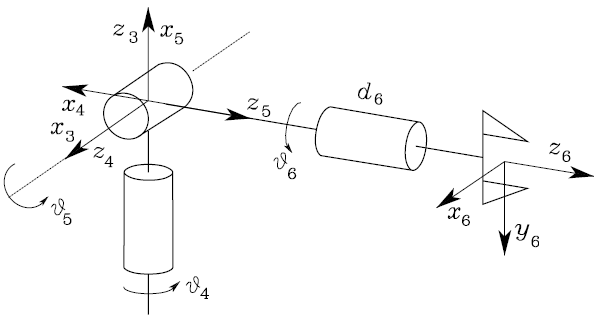
\includegraphics[width=0.55\textwidth]{figs/tipica_dh}
 	\caption[Manipulador tipo pulso esférico na convenção DH]
 	{Manipulador tipo pulso esférico na convenção DH \\
 	Fonte: adaptado	de~\cite{sciavicco2012modelling}}
 	\label{fig::tipica_dh}
\end{figure}

%
\begin{table}
\centering
\caption{Parâmetros DH do pulso esférico}
\label{tab::param_dh}
\begin{tabular}{@{}ccccc@{}}
\toprule
Elo & $a_i$ & $\alpha_i$ & $d_i$ & $\vartheta_i$ \\ \midrule
1   & 0     & $-\pi/2$   & 0     & $\vartheta_1$ \\
2   & 0     & $\pi/2$    & 0     & $\vartheta_2$ \\
3   & 0     & 0          & $d_6$ & $\vartheta_3$ \\ \bottomrule
\end{tabular}
\end{table}
%

\subsection{Cinemática Inversa}\label{sec::ikin}

O problema inverso, ou seja, encontrar o valor das juntas $\mathbf{q}$ que
satisfazem $\xi_{E}$, é feito pela análise da cinemática inversa. Logo:
%
\begin{equation} \label{eq::invq}
	\mathbf{q} = \mathcal{K}^{-1}(\xi_{E})
\end{equation}
%

A solução deste problema é de fundamental importância, porque transforma o
movimento desejado do efetuador, no espaço cartesiano, no valor correspondente
das juntas. Entretanto, \citet{sciavicco2012modelling} explicam por que o
problema da cinemática inversa é muito mais complexo:
%
\begin{itemize}
  \item As equações a serem resolvidas são geralmente não lineares, então nem
  sempre é possível obter uma solução de forma fechada;
  \item Múltiplas ou infitas soluções podem existir;
  \item Dependendo da estrutura cinemática do manipulador, pode não existir
  solução admissível.
\end{itemize}
%

De qualquer forma, para o manipulador de 6 gdl modelo MOTOMAN MH12 que é tratado
nesta pesquisa, há pelo menos 16 soluções admissíveis. Este número é
reduzido quando considerados os limites de ângulo das juntas.

Os manipuladores comerciais evoluiram mantendo uma estrutura cinematicamente
simples, muito em virtude da dificuldade da solução da cinemática inversa.
Há hoje diversas
técnicas para resolver o problema inverso, o que tem permitido explorar
manipuladores mais complexos. Para citar alguns exemplos:
método geométrico~\cite{spong2006robot}, 
subproblemas de Paden-Kahan~\cite{murray1994mathematical}, 
Jacobiano Transposto, Pseudoinversa e Mínimos Quadrados
Amortecido~\cite{buss2004introduction}.

O método escolhido para resolver a cinemática inversa foi o geométrico, devido à
sua simplicidade e ao manipulador MH12 possuir uma estrutura cinemática bastante
favorável à solução por este método. É demonstrado a seguir a metodologia
apresentada por \citet{spong2006robot}, utilizando o conceito de desacoplamento
cinemático, para chegar à solução da equação~\ref{eq::invq} pela abordagem
geométrica.


\subsubsection{Desacoplamento cinemático}

Para manipuladores que possuem 6 juntas, tal que as 3 últimas se interceptam no
mesmo ponto, é posível desacoplar a cinemática inversa em dois subproblemas mais
simples: cinemática inversa de posição e cinemática inversa de orientação. Ou
seja, para manipuladores de 6 gdl com pulso esférico, o problema torna-se
simplesmente encontrar a posição da interseção das 3 últimas juntas e a
orientação do pulso. Este conceito será utilizado para modelagem da cinemática
inversa do robô MOTOMAN MH12.

A Figura~\ref{fig::decoupling} ilustra o conceito de desacoplamento, onde
$\mathbf{p}_W$ refere-se a posição da origem do pulso esférico, $\mathbf{p}_E$ a
posição do efetuador e $\mathbf{d}_E$ a distância do efetuador para o pulso na direção
de orientada pelo efetuador.

\begin{figure}[h]
	\centering 
 	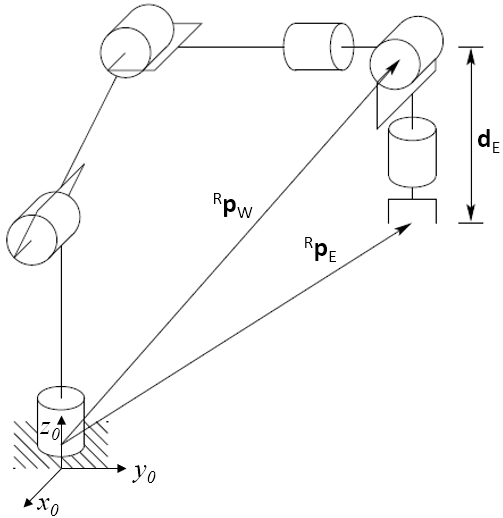
\includegraphics[width=0.45\textwidth]{figs/decoupling}
 	\caption[Desacoplamento cinemático]{Desacoplamento cinemático \\ Fonte:
 	adaptado de~\cite{spong2006robot}}
 	\label{fig::decoupling}
\end{figure}

Logo, pode-se definir a posição e orientação final da ferramenta acoplada ao
efetuador como:
%
\begin{equation}
	\mathbf{x}_{f} = \begin{bmatrix}
		\mathbf{p}_{f} \\ \boldsymbol{\Phi}_{f}
	\end{bmatrix}
	\label{eq::posf}	
\end{equation}
%
Onde $\mathbf{p}_{f}$ é um vetor das coordenadas da extremidade da ferramenta e
$\boldsymbol{\Phi}_{f}$ um vetor composto pelos ângulos de Euler que definem a
orientação da ferramenta.
%
\begin{align}
\mathbf{p}_{f} &= [x_f,y_f,z_f] \\
\boldsymbol{\Phi}_{f} &= [\phi,\theta,\psi]
\end{align}
%
Entretanto, a posição da ferramenta depende da posição do pulso, da orientação
e da distância entre o pulso e a ferramenta no referencial do pulso:
% 
\begin{equation} \label{eq::posfbib}
	\mathbf{p}_{f} = \mathbf{p}_{w} + [d_{x}, d_{y}, d_{z}]
\end{equation}
%
Logo, a solução da cinemática inversa, para o posição e orientação do pulso,
fornece a posição final da ferramenta, dada pela equação~\ref{eq::posfbib}.


\subsubsection{Solução da cinemática inversa de posicionamento}

Considerando-se apenas as 3 primeiras juntas do manipulador da
Figura~\ref{fig::decoupling}, e com auxílio das Figuras~\ref{fig::geom_pos_sup}
e \ref{fig::geom_pos_lat}, verifica-se as seguintes relações:
%
\begin{align}
	\theta_{1} &= \atantwo(x_c, y_c) \pm \atantwo(-\sqrt{r^2-d^2}, -d)
	\label{eq::theta1}\\
	\theta_{2} &= \atantwo(\sqrt{x_c^2+y_c^2-d^2}, z_c-d_1) - \atantwo(a_2+a_3
	c_3,a_3 s_3) \label{eq::theta2} \\
	\theta_{3} &= \atantwo(D, \pm \sqrt{1-D^2}) \label{eq::theta3}
\end{align}
%
Onde:
\begin{equation*}
		D = \frac{x_c^2+y_c^2-d^2 + (z_c-d_1)^2 - a_2^2 - a_3^2}{2a_2 a_3}
\end{equation*}
%
Os termos $x_c, y_c, z_c$ são a posição da extremidade do manipulador em que
é acoplado o pulso, $d$ é a distância de \textit{offset} da primeira junta,
$a_2$ e $a_3$ são os comprimentos dos elos. Utiliza-se a notação simplificada
das funções trigonométricas, portanto $s_2, c_2$, por exemplo, correpondem a
$\sin(\theta_2)$ e $\cos(\theta_2)$ respectivamente, o que valerá para todo o
texto.


\begin{figure}[h]
	\centering 
 	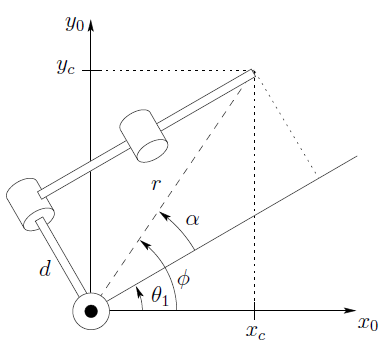
\includegraphics[width=0.45\textwidth]{figs/geom_pos_sup}
 	\caption[Vista na projeção xy do manipulador]{Vista na projeção xy do manipulador
 	\\ Fonte: adaptado de~\cite{spong2006robot}}
 	\label{fig::geom_pos_sup}
\end{figure}

\begin{figure}[h]
	\centering 
 	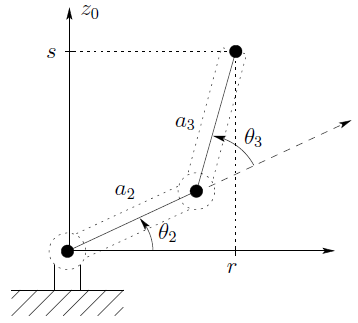
\includegraphics[width=0.45\textwidth]{figs/geom_pos_lat}
 	\caption[Vista na projeção xz do manipulador]{Vista na projeção xz do
 	manipulador \\ Fonte: adaptado de~\cite{spong2006robot}}
 	\label{fig::geom_pos_lat}
\end{figure}

Note-se que as equações encontradas fornecem 4 soluções de configuração do
manipulador para um mesmo ponto no espaço.

\subsubsection{Solução da cinemática inversa de orientação}

O problema da orientação inversa corresponde a encontrar os valores das 3 jnutas
do pulso para determinar a orientação desejada. A orientação desejada pode ser
definida pelos ângulos de Euler $\phi, \theta, \psi$ que transformam a
orientação do referencial inercial para a orientação final do referencial do
efetuador.
Então, basta encontrar os ângulos $\theta_4, \theta_5, \theta_6$ que satisfazem
a orientação desejada.

Logo, a equação que deve ser resolvida é a seguinte:
%
\begin{equation}
	R_3^6 = (R_0^3)^T R
\end{equation}


Pela matriz $R$ define-se a orientação final que se deseja alcançar pelo
efetuador.
Utilizando os ângulos de Euler para rotações em torno dos eixos ZYZ , fornece-se
a matriz que representa a orientação desejada:
%
\begin{equation} \label{eq::rzyz}
R_{zyz} = 
\begin{pmatrix}
c_\phi c_\theta c_\psi - s_\phi s_\psi & -c_\phi c_\theta s_\psi - s_\phi c_\psi & c_\phi s_\theta\\ 
s_\phi c_\theta c_\psi + c_\phi s_\psi & -s_\phi c_\theta s_\psi + c_\phi c_\psi & s_\phi s_\theta\\ 
-s_\theta c_\psi & s_\theta s_\psi & c_\theta
\end{pmatrix}
\end{equation}
%

A matriz transposta da rotação que leva do referencial inercial ao referencial
do pulso é:
%
\begin{equation}
	(R_0^3)^T = 
\begin{pmatrix}
c_1 c_{23} & -c_1 s_{23}  & s_1 \\ 
s_1 c{23} & -s_1 s_{23}  & -c_1 \\ 
s_{23} & c_{23}  & 0 
\end{pmatrix}
\end{equation}
%
E do pulso para o efetuador:
%
\begin{equation}
R_3^6 = 
\begin{pmatrix}
{ c_4} { c_5} { c_6}-{ s_4} {
 s_6}&-{ c_4} { s_5}&{ c_4} { c_5} { s_6}+{ c_6} {
 s_4}\\ { s_5} { c_6}&{ c_5}&{ s_5} {
 s_6}\\ -{ c_5} { c_6} { s_4}-{ c_4} {
 s_6}&{ s_4} { s_5}&-{ c_5} { s_4} { s_6}+{ c_4} {
 c_6}
\end{pmatrix} 
\end{equation}
%

Utilizando os resultados da cinemática inversa de posicionamento,
$\theta_1, \theta_2, \theta_3$ e definindo-se a orientação pelos ângulos de
Euler $\phi, \theta, \psi$ estão fornecidas no total 9 equações para 6
incógnitas: funções cossenos e senos de $\theta_4, \theta_5, \theta_6$.

Resolvendo-se o sistema, obtém-se:
%
\begin{align}
	\theta_4 &= \atantwo(c_1 c_{23} r_{13} + s_1 c_{23} r_{23} + s_{23} r_{33},
	-c_1 c_{23} r_{13} - s_1 c_{23} r_{23} + c_{23} r_{33} ) \label{eq::theta4} \\
	\theta_5 &= \atantwo(s_1 r_{13} - c_1 r{23}, \pm \sqrt{1- (s_1 r_{13} - c_1
	r_{23})^2}) \label{eq::theta5} \\
	\theta_6 &= \atantwo(-s_1 r{11} + c_1 r_{21}, s_1 r{12} - c_1 r_{22})
	\label{eq::theta6}
\end{align}
%
Onde $r_{ij}$ correspondem aos termos da matriz de orientação desejada, da
equação~\ref{eq::rzyz}.

Logo, o conjunto das equações~\ref{eq::theta1} a \ref{eq::theta3} e
\ref{eq::theta4} a \ref{eq::theta6} fornece as soluções da cinemática inversa,
pelo método geométrico, para os parâmetros de posição ($x_c, y_c, z_c$) e
orientação ($\phi, \theta, \psi$) desejados. 


\subsection{ Planejamento de trajetória} \label{sec::plan_traj}

Os parâmetros como posição, velocidade e orientação ao longo de um dado caminho
são impostos ao robô através de uma etapa chamada planejamento da trajetória.

% A importância de incluir corretamente os parâmetros da trajetória se
% deve ao fato de que são estes parâmetros que serão verificados ao se comparar
% os resultados do robô no modelo de base rígida aos resultados do modelo do robô
% sobre uma base flexível. 

Se a tarefa é, por exemplo, o processo de revestimento robótico por asperção de
uma superfície qualquer, o robô deve seguir uma trajetória de forma a cobrir
totalmente a superfície com o material.

Para cobertura autônoma de uma região, o campo de estudo da robótica é
denominado Planejamento de Caminho para Cobertura (ou CPP, de \textit{Coverage Path
Planning}). Consiste em determinar um caminho que passe por todos os
pontos de uma área ou volume de interesse, evitando
obstáculos~\cite{galceran2013survey}.

Neste contexto, uma técnica simples para cobertura completa é a chamada
Decomposição Celular Exata (\textit{exact cellular decomposition}) em que o
espaço a ser coberto é dividido em ``células'', tal que a união de todas as
células forma o espaço original~\cite{latombe1991exact}. Este método é útil para
automatizar a cobertura de superfícies por robôs móveis limpadores, veículos AUV
e robôs de pintura. A presente pesquisa utiliza tarefas de revestimento robótico
como estudo de caso, o que se aproxima de uma pintura de superfície.
Pela simplicidade das regiões simuladas, representadas por superfícies planas e
sem obstáculos, neste trabalho é empregado o método de decomposição celular de
\textit{boustrophedon}~\cite{choset2000coverage}. Outros métodos foram
desenvolvidos para regiões mais complexas, contendo obstáculos e fronteiras
singulares como: trapezoidal, \textit{based-morse} e
\textit{based-landmark}~\cite{galceran2013survey}.

O método de \textit{boustrophedon} consiste em dividir o espaço em células de
forma que o robô percorre cada célula com um movimento de zigue-zague e, uma vez
que se passa por todas as células, toda a área da superfície é considerada
coberta. A Figura~\ref{fig::boustrophedon} ilustra este conceito.

\begin{figure}[h]
	\centering 
 	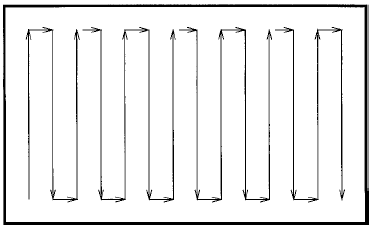
\includegraphics[width=0.45\textwidth]{figs/boustrophedon}
 	\caption[Cobertura pelo método de \textit{boustrophedon}]{Cobertura pelo
 	método de \textit{boustrophedon} \\ Fonte: adaptado de
 	de~\cite{choset2000coverage}}
 	\label{fig::boustrophedon}
\end{figure}

% exact cellular de composition
% Bountrophedon Path
% Coverage path planning
% covering salesman problem
% lawnmower problem

O sistema EMMA de revestimento por aspersão térmica, realiza a tarefa sobre uma
superfície suavemente curva, que representa o perfil hidráulico da pá de uma
turbina Kaplan. Como um dos requisitos do processo é manter a distância fixa
entre a pistola de revestimento e a pá, a trajetória não está restrita a apenas
um plano. \citet{8206216} apresentam uma metodologia que, dado um modelo CAD da
superfície e os parâmetros do processo, realiza-se pelo método RBF
(\textit{radial basis function}) a programação da trajetória para cobrir aquela
superfície. A Figura~\ref{fig::coat_blade} apresenta o modelo CAD da simulação
de revestimento robótico da pá pela metodologia proposta, onde a linha azul
representa o caminho percorrido sobre a superfície.

\begin{figure}[h]
	\centering 
 	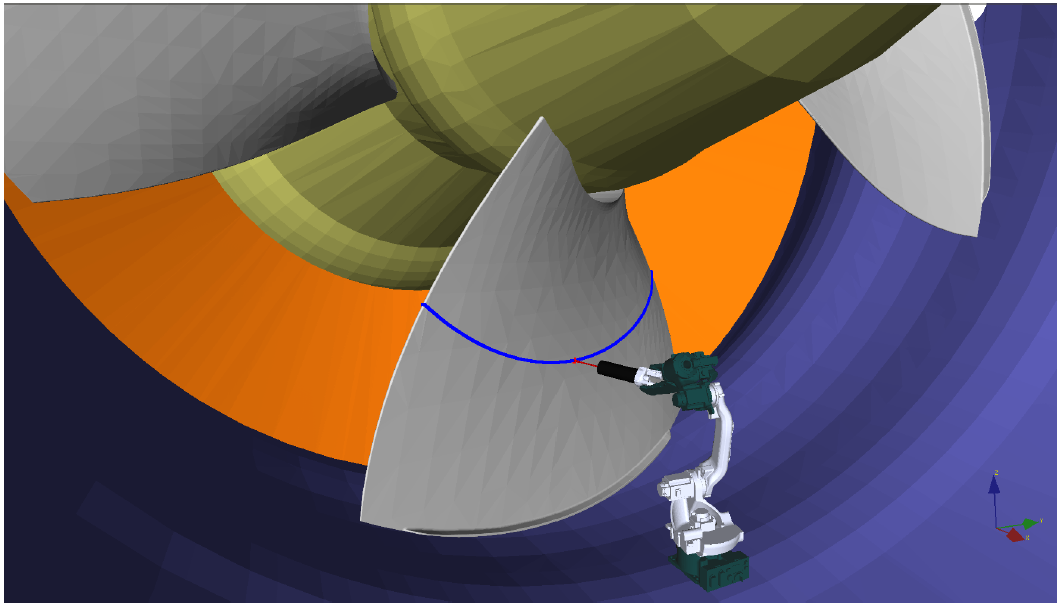
\includegraphics[width=0.75\textwidth]{figs/coat_blade}
 	\caption[Revestimento da face curva de uma pá]{Revestimento da face curva de
 	uma pá. \\Fonte: \citet{8206216}}
 	\label{fig::coat_blade}
\end{figure}

Devido à complexidade deste método, necessidade de ferramentas especiais e por
não acrescentar diferenças significativas para a discussão que se apresenta
neste trabalho, preferiu-se utilizar o método de \textit{boustrophedon} para
planejamento do caminho, considerando os requisitos do processo de revestimento
para planejamento da trajetória.



\subsection{Dinâmica e Equações de Movimento}

O estudo da dinâmica relaciona o movimento de um sistema multicorpos às forças
externas e de inércia que nele atuam. Nesta seção apresenta-se os métodos
clássicos para derivar as equações que regem o movimento do sistema. Outros
métodos também foram explorados historicamente, como as equações de
Hamilton~\cite{shabana2013dynamics},
Boltzmann-Hamel~\cite{papastavridis1994boltzmann} e
Gibbs-Appell~\cite{gibbsappell}.
 
\subsubsection{Equações de Newton-Euler}

A formulação de Newton-Euler são uma combinação das Leis de Newton para sistemas
de partículas, e das Leis de Euler, que introduziram os princípios da dinâmica
para corpos rígidos. 

Considerande-se novamente o sistema da Figura~\ref{fig::sist_refs}. Pela segunda
lei de Newton, tem-se que o somatório das forças $F$ que agem sobre o corpo B de
massa $m$ é igual a variação da quantidade de movimento $G$, ou seja:
%
\begin{equation} \label{eq::newton}
	\mathbf{F} = {^R}{\dot{\mathbf{G}}}^{B}
\end{equation}
%
Onde:
%
\begin{equation}
	\mathbf{G}^{B} = m {^R}\dot{\textbf{u}}^{B}
\end{equation}
%


De forma similar, as equações que descrevem a dinâmica do movimento angular são
determinadas, pela equação de Euler, como a variação da quantidade de movimento
angular $H$ igual ao somatório dos momentos externos, com respeito
ao centro de massa, que agem sobre o corpo.
%
\begin{equation} \label{eq::euler}
	\mathbf{M} = {^R}{\dot{\mathbf{H}}}^{B}
\end{equation}
%
Tal que a variação da quantidade de movimento angular pode ser escrita como:
%
\begin{equation}
	{^R}{\dot{\mathbf{H}}}^{B} = In_B \cdot {^R}\dot{\boldsymbol{\alpha}}^{B} +
	{^R}\boldsymbol{\omega}^{B} \times In_B \cdot {^R}\boldsymbol{\omega}^{B}
\end{equation}
%
Onde $In_B$ representa o tensor de inércia do corpo B, com respeito ao centro de
massa e alinhado ao sistema de coordenadas local.

As equações~\ref{eq::newton} e \ref{eq::euler} fornecem as 6 equações de
movimento do sistema MBS da Figura~\ref{fig::sist_refs}. Para um caso geral, e
de sistemas de corpos conectados, são formuladas as equações de movimento de
cada corpo, o número de graus de liberdade é reduzido e parte destas 6 equações
de movimento são usadas para determinar as forças e momentos de
contato~\cite{tenenbaum2006fundamentals}.


% The Newton-Euler laws are a combination of the second law of Newton
% (sum of forces equals change of momentum) and Euler's law for the
% change of angular momentum. Both laws lead for an n-body system to a
% set of 6n second-order differential equations describing the dynamic
% behaviour of the system. ``Sol, p.7''

% The dynamics of multibody systems is based on classical mechanics. The most
% simple element of a multibody system is a free particle which can be treated by
% Newton’s equations published in 1686 in his “Philosophiae Naturalis Principia
% Mathematica” [111]. The principal element, the rigid body, was introduced in 1775
% by Euler in his contribution entitled “Nova methodus motum corporum rigidarum
% determinandi” [43]. For the modeling of constraints and joints, Euler already used
% the free body principle resulting in reaction forces. The equations obtained are
% known in multibody dynamics as Newton–Euler equations.  ``Schielen, p.149''

%\subsubsection{Princípio de d'Alembert}

% A system of constrained rigid bodies was considered in 1743 by d’Alembert in his
% “Trait´e de Dynamique” [32] where he distinguished between applied and reaction
% forces. D’Alembert called the reaction forces “lost forces” having the principle
% of virtual work in mind. A mathematical consistent formulation of d’Alembert’s
% principle is due to Lagrange [89] combining d’Alembert’s fundamental idea with
% the principle of virtual work. As a result a minimal set of ordinary
% differential equations (ODE) of second order is found. ``Schielen, p.150''


\subsubsection{Equações de Lagrange}

O método Lagrangeano requer as propriedades de energia do sistema mecânico para
computar as equações de movimento. Esta técnica tem a vantagem de precisar
apenas das energias cinética e potencial do sistema e,
segundo~\citet{murray1994mathematical}, tende a ser menos sujeita a erros do que
somar as forças inerciais, de Coriolis, de atuadores, e outras que atuam nos
elos do robô, por exemplo.

Para escrever as equações de movimento, deve-se definir primeiro o
Lagrangeano, $L$:
%
\begin{equation}
	L(q, \dot{q}) = T(q, \dot{q}) - V(q)
\end{equation}
%
Onde, $T$ é a energia cinética, $V$ a energia potencial do sistema e
$q$ as coordenadas generalizadas.

Então as equações de movimento do sistema, em notação vetorial, podem ser dadas
por:
%
\begin{equation}
	\frac{\mathrm{d} }{\mathrm{d} t}\frac{\partial L}{\partial \mathbf{\dot{q}}} -
	\frac{\partial L}{\partial \mathbf{q}} = \boldsymbol{\Upsilon}
\end{equation}
%
Onde $\boldsymbol{\Upsilon}$ são as forças externas associadas a cada
coordenada generalizada do sistema.

O método de Lagrange é interessante sobretudo porque reduz o número de equações
necessárias, de $n$, o número de partículas do sistema, para $m$, o número de
coordenadas generalizadas. Em contrapartida ao método de Newton-Euler, este
não requer a consideração das forças internas ou de restrição do sistema MBS, o
que reduz o número de equações a serem resolvidas.



% A systematic analysis of constrained mechanical systems was established in
% 1788 by Lagrange [89], too. The variational principle applied to the total kinetic
% and potential energy of the system considering its kinematical constraints and the
% corresponding generalized coordinates result in the Lagrangian equations of the
% first and the second kind. Lagrange’s equations of the first kind represent a set of
% differential-algebraical equations (DAE) while the second kind leads to a minimal
% set of ordinary differential equations (ODE). ``Schielen, p.150''

\subsection{Sophia-Maple e Método de Kane}\label{sec::sophia_kane}

\subsubsection{Kane}

O método de Lagrange tem a vantagem de eliminar as forças que não realizam
trabalho, mas a desvantagem de ter que lidar com cálculo diferencial das
equações de energia. O método de Newton-Euler introduz as forças de contato e
restrição, que devem ser resolvidas para chegar às equações de movimento, no
entanto, apenas relações de cálculo vetorial são suficientes para fornecer o
modelo cinemático completo do sistema. Já o método de Kane pode ser
considerado como tendo as vantagens de ambos, mas sem as desvantagens.

No artigo que originou o método, \citet{kane1965derivation} resumem
as principais características da metodologia: 
%
\begin{enumerate*}[label=\emph{\alph*})]
	\item automaticamente elimina as forças que não realizam trabalho;
	\item aplicável a sistemas holonômicos e não-holonômicos;
	\item conduz diretamente a equações de diferenciais de primeira ordem.
\end{enumerate*}

O tempo computacional necessário para resolver um sistema de equações cresce
quadraticamente com a dimensão do sistema e as forças e torques de restrição
podem ser grandes, o que leva a passos de integração pequenos para prevenir a
divergência da solução~\cite{stoneking2013implementation}. Neste sentido, o
método agora detalhado por~\citet{kane1985dynamics} tornou-se popular para
derivar as equações de movimento de sistemas MBS, sobretudo porque fornece um
número mínimo de equações.

As equações de Kane são normalmente apresentadas como o seguinte conjunto de
equações:
%
\begin{equation} \label{eq::kane}
	F_r + F_r^{*} = 0 \qquad, r = 1,\ldots,n
\end{equation}
%
Onde $n$ é o número de graus de liberdade, $F_r$ são as forças externas
generalizadas e $F_r^{*}$ as forças de inércia generalizadas, que podem ser
expressas para um conjunto de N corpos, respectivamente por:
%
\begin{gather}
%eq1
	F_r = \sum_{k=1}^{N}(\boldsymbol{\omega}_r^k \cdot \mathbf{T}_k) +
\sum_{k=1}^{N}(\mathbf{v}_r^k \cdot \mathbf{F}_k) \\
%eq2
	F_r^{*} = \sum_{k=1}^{N}\left[\boldsymbol{\omega}_r^k \cdot (-I_k
\boldsymbol{\alpha}_k - \boldsymbol{\omega}_k \times \mathbf{H}_k)\right] +
\sum_{k=1}^{N}\left[ \mathbf{v}_r^k \cdot (\mathbf{F} - m \mathbf{a})_k \right]
= 0
\end{gather}
%

Os vetores $\boldsymbol{\omega}_r$ e $\mathbf{v}_k$ são respectivamente as
\emph{velocidades parciais angulares} e \emph{velocidades parciais lineares}. De
forma mais geral, pode-se encontrar um vetor de velocidades generalizadas e
deste obter o chamado hiperplano tangente.
Este plano é uma generalização da superfície que restringe o movimento do
sistema MBS e é obtido pela diferenciação das velocidades com respeito às
coordenadas generalizadas do sistema. As velocidades parciais são calculadas
pela expressão das velocidades generalizadas, na equação~\ref{eq::velgen}. O
termo explicitado na equação~\ref{eq::tau} define o vetor tangente associado a
k-ésima coordenada generalizada.
%
\begin{gather}
%eq1
	\mathbf{v} = \frac{\mathrm{d} \mathbf{p}}{\mathrm{d} t} = \sum_{k=1}^{N}
	\dot{q_{k}} \frac{\partial p}{\partial q_{k}} + \frac{\mathrm{d}
	q_{k}}{\mathrm{d} t} \label{eq::velgen}\\
%eq2
	\frac{\partial p}{\partial q_{k}} = \tau_{k} \label{eq::tau}
\end{gather}
%

O hiperplano tangente, $\tau$, projeta a equação de equilíbrio dinâmico de
Newton-Euler, para ao mesmo tempo eliminar as forças que não realizam trabalho e
obter-se um número mínimo de equações das forças de inércia e externas
generalizadas.
As equações cinemáticas diferenciais~\ref{eq::kde} (ou kde, de \textit{kinematic
differential equations}) permitem transformar o sistema de equações diferenciais
de segunda ordem, em dois conjuntos de primeira ordem.
%
\begin{equation} \label{eq::kde}
	u_r = \dot{q}_r \qquad, r = 1,\ldots,n
\end{equation}
%

As equações~\ref{eq::kane} e \ref{eq::kde} formam, portanto, um sistema de
equações de diferenciais ordinárias não-lineares de primeira ordem, que
representam as equações de movimento do sistema MBS.


\subsubsection{Sophia e notação de Lesser} \label{sec::lesser}

Sophia é um conjunto de rotinas implementado para Maple. O programa foi
desenvolvido pelo professor Martin Lesser do KTH Royal Institute of Technology,
Suécia, e sua sintaxe e utilização está bem detalhada no livro intitulado
``\textit{The Analysis of Complex Nonlinear Mechanical
Systems}''\cite{lesser1995analysis}. Sophia foi desenhado especificamente para
modelagem simbólica de sistemas mecânicos multicorpos, e oferece uma forma
sistemática e simples de se chegar às equações de movimento através do método de
Kane. Posteriormente foram implementadas por \citet{lennartsson1999efficient}
melhorias no programa para eficiência algébrica e também o pacote
\texttt{exmex}, para exportação das equações de movimento para solução numérica
no MATLAB ou Octave.

Para auxiliar a compreensão da notação utilizada por Lesser no Sophia, faz-se
uma pequena revisão dos principais termos utilizados pelo programa para lidar
eficientemente com a álgebra de vetores e tensores.

\medskip \noindent
\texttt{- Evector} -- No Sophia, os vetores são compostos por objetos de duas
partes:
seu conjunto de componentes e a identificação do sistema de coordenadas a que se
refere. Este objeto é chamado de \texttt{Evector}, tal que 'E' indica que este
pertence ao espaço tridimensional Euclidiano. Como exemplo, o vetor posição de
um ponto paralelo ao vetor unitário $\mathbf{a}_1$ a uma distância $L1$ é
definido como um \texttt{Evector} da seguinte forma:

\medskip \texttt{> Evector(L1,0,0, A);	} \medskip

\noindent O que retorna: \texttt{[[L1, 0, 0], A]} \medskip


\medskip \noindent
\texttt{- chainSimpRot} -- Esta função representa o método mais direto para se
relacionar os referenciais como uma sequência de rotações simples. Para
isso cria-se uma lista contendo os referenciais relacionados, o eixo de rotação
e a variável, ou coordenada generalizada associada àquela rotação pela função
\texttt{chainSimpRot} que reune em uma lista, a lista de rotações. Por exemplo:

\medskip \texttt{> chainSimpRot([N, A, 3, q1], [A, B, 3, q2]);	}
\medskip

Desta forma, define-se internamente as matrizes de rotação entre os referenciais
A, B e N. Estas relações são utilizadas para relacionar os referenciais e
permitir a diferenciação dos 'E' vetores.

\medskip \noindent \texttt{- DiffFrame} -- Para diferenciar os 'E' vetores em
função de qualquer variável em relação a qualquer referencial, a função
\texttt{DiffFrame} (ou sua variação \texttt{\&fdt}) é utilizada. Como argumento
são fornecidos o vetor, a variável e o referencial.
Esta função é útil para derivar os vetores posição e calcular as velocidades
lineares.

\medskip \noindent
\texttt{- \&av} -- A velocidade angular entre dois referenciais pode ser
facilmente calculada pela função \texttt{\&av}. Como exemplo, para calcular o
vetor $^N\boldsymbol{\omega}^B$:

\medskip \texttt{> wNB := N \&av B; } \medskip

\medskip \noindent
\texttt{- Edyad} -- Assim como os 'E'vetores, os tensores são compostos por dois
termos: componentes e um referencial associado.

\medskip \noindent
\texttt{- \&o} e \texttt{\&xx} -- O produto escalar entre 'E' vetores e 'E'
tensores pode ser obtido com a função \texttt{\&o}.
Já o produto vetorial é obtido pela função \texttt{\&xx}. Em ambos os casos, o
resultado mantém a estrutura da notação e não requer que os vetores ou tensores
estejam escritos no mesmo referencial, lidando automaticamente com as
transformações necessárias.

\medskip \noindent
\texttt{- SKvector} -- Os super \texttt{Kvector} ou \texttt{SKvector} são
vetores formados por uma lista de 'K' vetores. Como exemplo, o vetor das
velocidades generalizadas é um \texttt{Kvector}, no sentido de que é uma lista
de \texttt{Evector} e o vetor do hiperplano tangente, $\tau$, é um
\texttt{SKvector}, por ser formado por uma lista de \texttt{Kvector}.
%
\begin{equation}
\tau = 
\begin{bmatrix}
\boldsymbol{\tau}_1\\ 
\vdots\\ 
\boldsymbol{\tau}_n
\end{bmatrix}
=
\begin{bmatrix}
\begin{bmatrix}
\boldsymbol{\tau}_1^1\\ 
\vdots\\ 
\boldsymbol{\tau}_1^k
\end{bmatrix}\\ 
\vdots\\ 
\begin{bmatrix}
\boldsymbol{\tau}_n^1\\ 
\vdots\\ 
\boldsymbol{\tau}_n^k
\end{bmatrix}\\ 
\end{bmatrix}
\end{equation}
%

Sophia demonstra duas grandes vantagens. A primeira é que reduz a necessidade de
lidar com a manipulação de expressões algébricas extensas. A segunda é a
sistematização da modelagem do sistema mecânico, por meio de declarações simples
e objetivas do problema.



% -.~.-.~.-.~.-.~.-.~.-.~.-.~.-.~.-.~.-.~.-.~.-
\section{Análise dinâmica de estruturas}

O projeto e análise de estruturas que estão sujeitas a carregamentos dinâmicos
consiste em assumir idealizações e simplificações da estrutura física a fim de
representá-la como um modelo analítico ou matemático. \citet{paz2012structural}
resume estas idealizações nos seguintes grupos: 
%
\begin{enumerate*}[label=\emph{\alph*})]
	\item \emph{material}: simplificações e premissas como homogeneidade e
	isotropia;
	\item \emph{carregamento}: as forças consideradas concentradas em pontos
	específicos, repentina ou periodicamente aplicadas;
	\item \emph{geometria}: perfis extrudados, ou vigas são normalmente
	considerados elementos unidirecionais, podem ser discretizadas em nós.
\end{enumerate*}

Para ilustrar o projeto e análise dinâmica de estruturas,
\citet{craig2006fundamentals} ilustram bem as etapas necessárias, como pode ser
visto no diagrama da Figura~\ref{fig::analise_estrut}. Estes passos guiam a
modelagem e verificação do projeto para base do robô no método proposto nesta
pesquisa.

\begin{figure}[h]
	\centering 
 	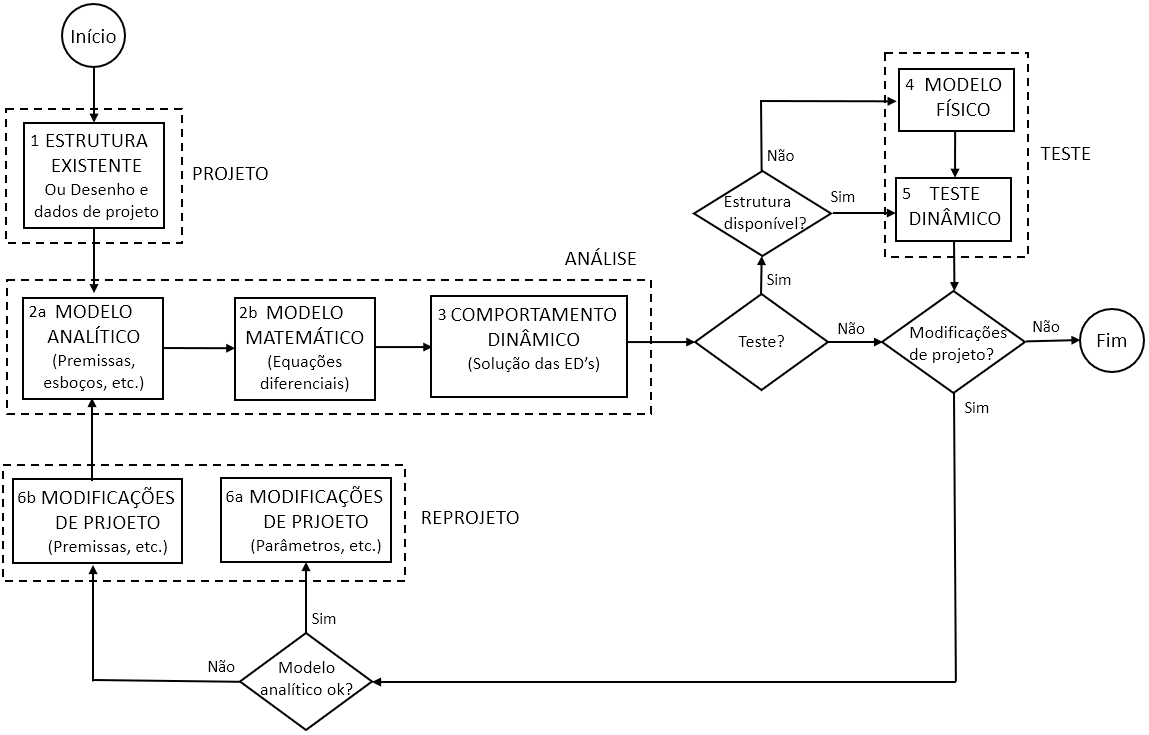
\includegraphics[width=0.98\textwidth]{figs/analise_estrut}
 	\caption[Diagrama de investigação da dinâmica de estruturas]{Diagrama de
 	investigação da dinâmica de estruturas. \\Fonte:
 	adaptado de \cite{craig2006fundamentals}}
 	\label{fig::analise_estrut}
\end{figure}

As equações de movimento que regem o comportamento dinâmico dependem da massa,
rigidez e amortecimento da estrutura, de acordo com a expressão:
%
\begin{equation} \label{eq::eqmov_structural}
	M \ddot{\mathbf{q}} + C \dot{\mathbf{q}} + K \mathbf{q} = \mathbf{f}(t)
\end{equation}
%

Logo, deve-se haver uma forma de fornecer estes parâmetros ao modelo matemático
da estrutura, a fim de realizar a análise do seu comportamento dinâmico.


\subsection{Rigidez} \label{sec::rigidez}

A rigidez relaciona o deslocamento, devido a deformações elásticas da estrutura,
ao carregamento imposto.
Para uma estrutura de $n$ graus de liberdade, e coordenadas generalizadas $q$
associadas aos graus de liberdade da estrutura, podemos escrever:
%
\begin{equation} \label{eq::rigidez}
	\mathbf{f} = K \mathbf{q}
\end{equation}
%
O termo $K$ é uma matriz quadrada e simétrica que representa a matriz de
coeficientes de influência de rigidez da estrutura.
\citet{turner23stiffness} apresentaram um método para obter a rigidez total de
uma estrutura, pela soma da rigidez de unidades discretizadas, que ficou
conhecido como método da rigidez direta (ou \textit{direct stiffness method}).

Este método permite avaliar a relação entre força e deslocamento de qualquer nó
do modelo analítico da estrutura e montar a matriz de rigidez associada aos
graus de liberdade daquele ponto. Os coeficientes de influência $k_{ij}$ da
matriz $K$ podem ser calculados coluna a coluna. Para isso, são realizados
deslocamentos prescritos unitários na direção $j$ de cada grau de liberdade do
nó e calculadas as forças de reação na direção $i$ àquele deslocamento. As
forças e momentos de reação calculadas são exatamente os necessários para manter
a configuração dada pelo deslocamento prescrito na direção $i$, sem permitir
nenhum deslocamento na direção $j$. Como exemplo, considere-se o modelo
analítico bidimensinoal da Figura~\ref{fig::ex_stiff_analitico}.

\begin{figure}[h]
	\centering 
 	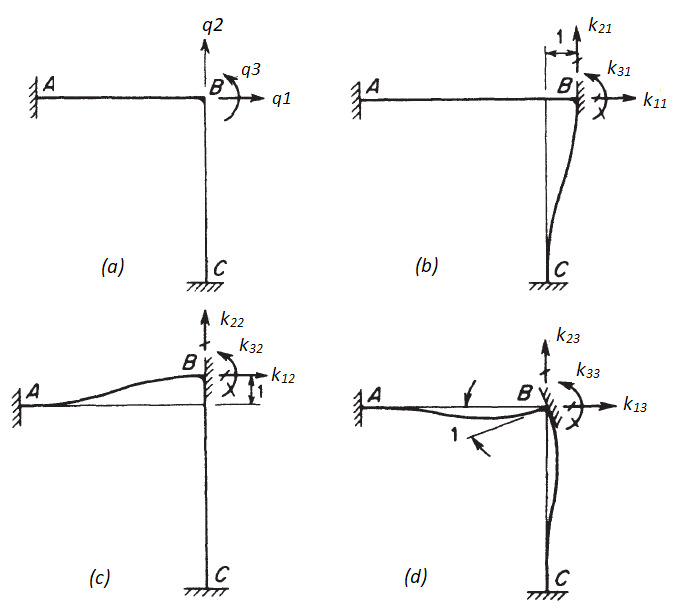
\includegraphics[width=0.80\textwidth]{figs/ex_stiff_analitico}
 	\caption[Exemplo de estrutura analítica para matriz de rigidez]{Exemplo de estrutura
 	analítica para matriz de rigidez: (a)
 	modelo analítico; (b) deslocamento unnitário em q1; (c) deslocamento
 	unitário em q2; (d) deslocamento unitário em q3. Fonte:
 	adaptado de \cite{weaver2012matrix}}
 	\label{fig::ex_stiff_analitico}
\end{figure}

No exemplo, o ponto B da estrutura possui 3 graus de liberdade: 2 translacionais
e um rotacional, representados por $q1, q2, q3$. São aplicados deslocamentos
unitários em cada direção e restringidos os deslocamentos nas outras direções em
cada caso. De acordo com a equação~\ref{eq::rigidez}, pode-se calcular cada
coeficiente de rigidez $k_{ij}$ como:
%
\begin{equation}
	k_{ij} = \frac{f_i}{q_j}
\end{equation}
%
Onde $f_i$ são as cargas de reação ao deslocamento prescrito em cada caso. A
matriz de rigidez será portanto $K_{3\times3}$, função das propriedades de
material e geometria dos elementos AB e BC e das condições de contorno.

Calcular analiticamente a matriz de rigidez por este método é viável para
estruturas simples. Para estruturas mais complexas, tridimensionais, com
restrições, carregamentos e contatos variados, será utilizado um modelo
numérico, resolvido por Análise de Elementos Finitos, utilizando o método
apresentado para obter a matriz de rigidez associada a um ponto de interesse da
estrutura.


\subsection{Amortecimento} \label{sec::amortecimento}

Do ponto de vista prático, as propriedades de amortecimento de um sistema
raramente são conhecidas, ao contrário das propriedades de rigidez e inércia.
A abordagem mais comum é tratar o amortecimento como viscoso, ou seja, as forças
de amortecimento dependem apenas das velocidades generalizadas, como considerado
na equação~\ref{eq::eqmov_structural}.
Porém, é necessário um método para obter a matriz de amortecimento da estrutura,
a fim de poder utilizá-la no modelo matemático matricial.

\subsubsection{Amortecimento de Rayleigh} \label{sec::amortecimento_revbib}

Também conhecido como amortecimento proporcional, este método consiste em
definir a matriz de amortecimento por meio de dois parâmetros $\alpha$ e
$\beta$, proporcionais às matrizes de inércia e rigidez. 
%
\begin{equation}
	C = \alpha M + \beta K	
\end{equation}
%

Ainda assim, os coeficientes devem ser encontrados. Pode ser verificado
em~\cite{craig2006fundamentals} que a transformação ortogonal da matriz $C$
fornece a equação do amortecimento modal como função dos coeficientes
de Rayleigh:
%
\begin{equation} \label{eq::xir}
	\xi_r = \frac{1}{2}\left(\frac{\alpha}{\omega_r} + \beta \omega_r\right )
\end{equation}
%
Onde $\xi_r$ e $\omega_r$ são respectivamente o amortecimento modal e a
frequência natural do r-ésimo modo de vibração. Artigos de
\citet{chen1996estimation}, \citet{adhikari2004rayleigh} e
\citet{schwarz2013proportional} apresentam metodologias para ajustar os
coeficientes de Rayleigh aos resultados experimentais de análise modal. Pelo
desenvolvimento de Schwarz, utilizando-se o método dos erros mínimos quadrados,
obtém-se a seguinte equação para os coeficientes de Rayleigh:
%
\begin{equation} \label{eq::brian}
	\begin{bmatrix}
	\alpha \\
	\beta
	\end{bmatrix}
= 2
	\begin{pmatrix}
	N & {\sum\limits_{i=1}^{N}\Omega_i^{2}} \\ 
	{\sum\limits_{i=1}^{N}\Omega_i^{2}} &
	{\sum\limits_{i=1}^{N}\left(\Omega_i^{2}\right)^2}
	\end{pmatrix}^{-1}
	\begin{bmatrix}
	\sum\limits_{i=1}^{N}\xi_i \\ 
	\sum\limits_{i=1}^{N}\xi_i \Omega_i^2
	\end{bmatrix}
\end{equation}
%
Onde $\Omega_i$ são as frequências de ressonância e $\xi_i$ os amortecimentos
modais obtidos experimentalmente para o i-ésimo modo; e $N$ representa o número
de ressonâncias na faixa medida.

\subsection{Análise modal experimental} \label{sec::modal_analysis}

A análise modal pode ser definida como um processo onde descreve-se uma
estrutura em termos de suas características naturais, que são a frequência,
amortecimento e modo -- suas propriedades
dinâmicas~\cite{avitabile2001experimental}.

Os modos de vibração, ou ressonâncias, são propriedades inerentes da estrutura,
determinadaos pela massa, rigidez, amortecimento e condições de contorno. Cada
modo é definido por uma frequência natural, amortecimento modal e forma.
Especificando-se o movimento de dois ou mais pontos na estrutura, define-se a a
Forma de Deflexão Operacional (ou ODS, de \textit{Operational Deflection
Shape})~\cite{schwarz1999experimental}, o que fornece uma visualização do
movimento e forma de vibração de uma determinada estrutura ou equipamento.
.

\citet{rao2011mechanical} resumem o aparato experimental necessário para análise
modal por ensaio de vibrações:
%
\begin{enumerate}
  \item Um excitador, que aplica uma força de entrada conhecida. Pode ser um
  \textit{shaker} ou um martelo instrumentado, por exemplo;
  \item Um transdutor para converter o sinal físico de movimento da estrutura em
  sinal elétrico, como acelerômetro por exemplo;
  \item Um analisador com condicionador de sinal, para realizar tarefas de
  processamento de sinais e análise modal utilizando um \textit{software} compatível. O tipo mais
  utilizado é o analisador pela transformada rápida de Fourier (ou FFT, de
  \textit{fast fourier transform}). 
\end{enumerate}

A análise modal requer que algumas considerações sejam válidas.
\citet{dossing1988structural} explica que a principal premissa é a linearidade.
Logo, a resposta será sempre proporcional à excitação. Esta consideração implica
também nas seguintes propriedades:
%
\begin{itemize}	
  \item \emph{Superposição}. Uma FRF medida não depende do tipo de excitação, desde que
  seja conhecida;
  \item \emph{Homogeneidade}. A FRF independe do nível de excitação.
  \item \emph{Reciprocidade}. A FRF medida entre quaisquer 2 gdl's independe
  de quem é a excitação e quem é a resposta. Isto implica que a matriz
  $H(\omega)$ é simétrica.
\end{itemize}

\subsubsection{Teste com martelo instrumentado}

Este método é o mais popular para teste modal utilizado hoje, pela rapidez,
conveniência e baixo custo, podendo ser utilizado em uma grande variedade de
estruturas e máquinas. A Figura~\ref{fig::impact_testing} apresenta as etapas de
uma análise modal com martelo instrumentado.

\begin{figure}[h]
	\centering 
 	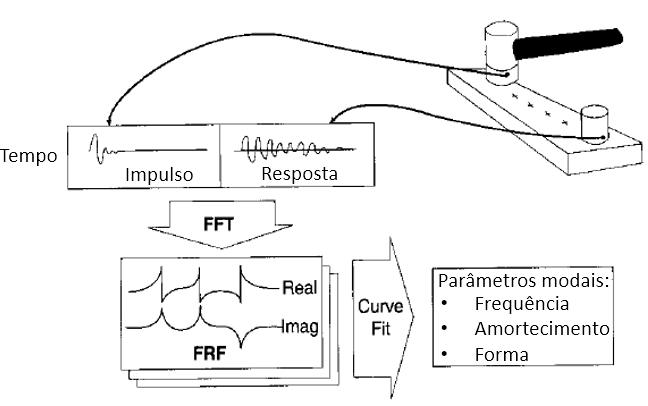
\includegraphics[width=0.60\textwidth]{figs/impact_testing}
 	\caption[Análise modal com martelo instrumentado]{Análise modal com martelo
 	instrumentado \\
 	Fonte: adaptado de \cite{schwarz1999experimental}}
 	\label{fig::impact_testing}
\end{figure}

A forma da resposta em frequência da excitação do impacto depende da massa e
rigidez do martelo e da estrutura. Segundo~\citet{rao2011mechanical}, a faixa
útil de frequência da excitação é limitada, de modo que a partir de um certo
valor a estrutura não recebe energia suficiente para excitar modos de frequência
mais altas. Normalmente, este valor é limitado a uma queda de amplitude da
excitação entre $10~dB$ a $20~dB$. A Figura~\ref{fig::range_hammer}
apresenta um resultado típico da resposta em frequência da excitação por impacto, indicando a
faixa útil a ser considerada.

\begin{figure}[h]
	\centering 
 	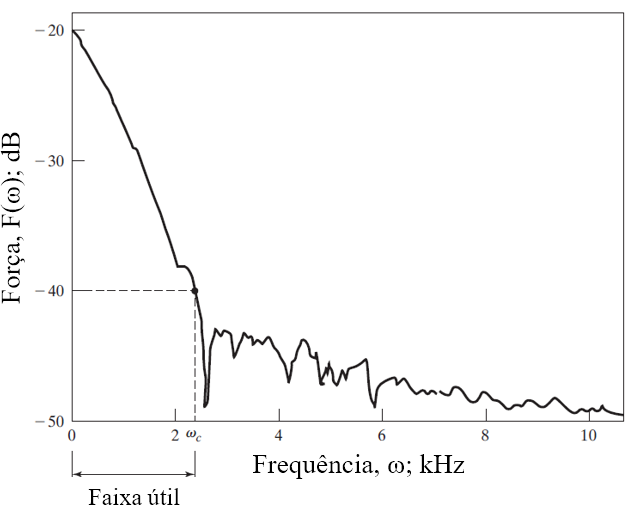
\includegraphics[width=0.55\textwidth]{figs/range_hammer}
 	\caption[Resposta em frequência de um impacto por martelo
 	instrumentado]{Resposta em frequência de um impacto por martelo
 	instrumentado \\
 	Fonte: adaptado de \cite{rao2011mechanical}}
 	\label{fig::range_hammer}
\end{figure}

Logo, para estruturas grandes e pesadas, normalmente são necessários martelos de
massa elevada, a fim de fornecer energia suficiente para excitar uma faixa
considerável de frequência.


\subsubsection{Função de Resposta em Frequência}

A Função de Resposta em Frequência, ou FRF, descreve a relação entre a saída e
entrada entre 2 pontos numa estrutura como função da frequência, sendo numa
análise de vibrações, a aceleração de saída, em relação à força de excitação de
entrada. \citet{avitabile2001experimental} acrescenta que a FRF contém
informações do sistema com respeito a frequências e amortecimento e uma coleção
de FRF's contém informação com respeito à forma, ou modos. E conclui: é a medida
mais importante relacionada à análise modal experimental. A
Figura~\ref{fig::diagrama_frf} demonstra a representação da função FRF,
$H(\omega)$ em diagrama de bloco.

\begin{figure}[h]
	\centering 
 	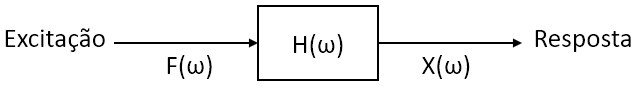
\includegraphics[width=0.65\textwidth]{figs/diagrama_frf}
 	\caption{Diagrama de bloco de uma FRF de um sistema mecânico}
 	\label{fig::diagrama_frf}
\end{figure}

Normalmente os dados são obtidos em amostras e são computadas as médias, para
obter-se a FRF e a Coerência. A função de coerência é usada como
ferramenta para avaliação da qualidade dos dados, identificando o quanto o dado de saída se
relaciona com o de entrada~\cite{avitabile2001experimental}. A coerência
$\beta(\omega)$ mede o ruído presente no sinal, sendo portanto $\beta = 0$ ruído
puro e $\beta \approx 1$ como alta correlação dos sinais de entrada e saída,
livres de ruído. A Figura~\ref{fig::coerencia} apresenta um resultado típico da
análise modal, sobrepondo a magnitude da FRF, o espectro de frequência da
excitação e a coerência. Note-se que a partir de aproximadamente $400~Hz$, a
coerência diminiu drasticamente, e portanto, o resultado a partir desta
frequência é muito ruidoso e não deve ser considerado útil.

\begin{figure}[h]
	\centering 
 	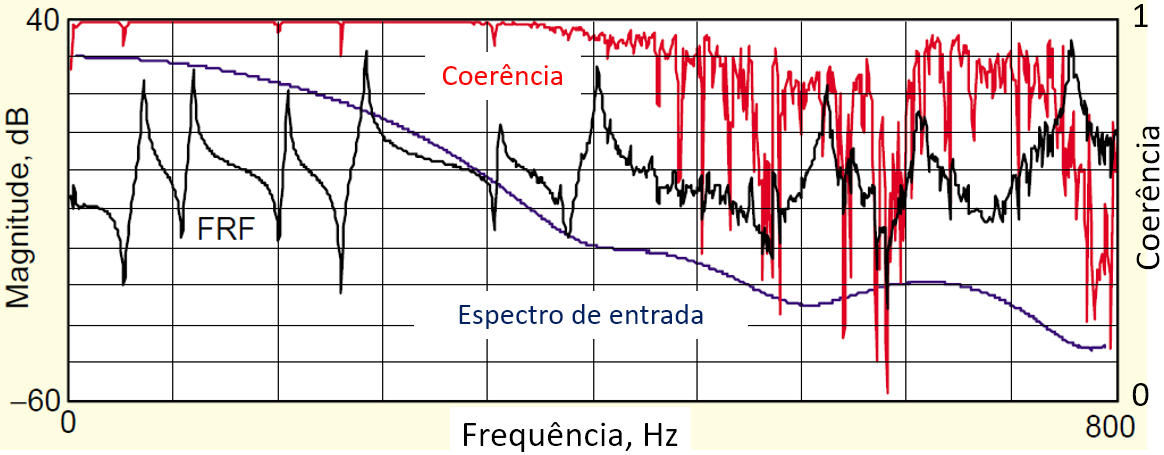
\includegraphics[width=0.85\textwidth]{figs/coerencia}
 	\caption[Resultados típicos de medição da excitação, FRF e
 	coerência]{Resultados típicos de medição da excitação (linha azul), FRF
 	(linha preta) e coerência (linha vermelha).	Fonte: adaptado de
 	\cite{avitabile2001experimental}}
 	\label{fig::coerencia}
\end{figure}

Cada FRF medida é associada a um único gdl de entrada com um único gdl de saída.
As FRF's são indicadas por dois índices, $i$ representando o gdl da excitação e
$j$ o gdl da saída.
%
\begin{equation}
	H_{ij} = \frac{X_i}{F_j}
\end{equation}

Logo, a função de resposta em frequência pode ser representada por uma matriz $n
\times n$, onde $n$ é o número de graus de liberdade medidos da estrutura.
Estruturas reais têm infitos graus de liberdade, mas devido a restrições de
tempo e custo, apenas um número finito e relativamente pequeno é medido.

Devido às propriedades de linearidade citadas anteriormente, apenas uma linha ou
uma coluna da matriz de resposta em frequência bastam para fornecer toda a
informação necessária para a análise dos parâmetros modais de uma estrutura.


\subsubsection{Determinação dos parâmetros modais}

Um método simples de encontrar os parâmetros modais é,
segundo~\citet{rao2011mechanical} utilizar a abordagem de
único-grau-de-liberdade. Consistem em dividir o gráfico da FRF em faixas de
frequência de modo a cada faixa englobar um único pico. Isto implica que a
função de resposta naquela faixa é dominada por um único modo. Logo, cada pico
representará uma ressonância, associada aquela frequência no pico. Isto está
representado na Figura~\ref{fig::tipical_frf}

\begin{figure}[h]
	\centering 
 	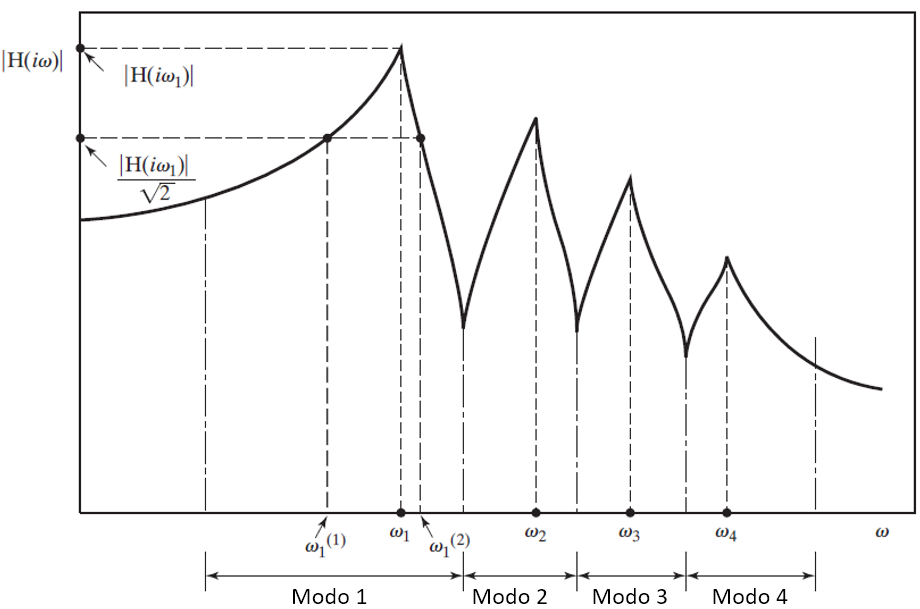
\includegraphics[width=0.85\textwidth]{figs/tipical_frf}
 	\caption[Resultado para determinação dos parâmetros modais]{Resultado para
 	determinação dos parâmetros modais \\ Fonte: adaptado de
 	\cite{rao2011mechanical}}
 	\label{fig::tipical_frf}
\end{figure}

O amortecimento modal também pode ser calculado pelo resultado da
Figura~\ref{fig::tipical_frf}, de acordo com a expressão:
%
\begin{equation}
	\zeta_j = \frac{\omega_j^{(2)} - \omega_j^{(1)}}{2 \omega_j}
\end{equation}
%
Onde $\omega_j^{(2)}$ e $\omega_j^{(1)}$ são conhecidos como frequências de
meia-banda situados em cada lado da frequência de ressonância $\omega_j$, de
forma que satisfazem a seguinte relação:
%
\begin{equation}
	\left | H(i\omega_j)^{(1)}) \right | = \left | H(i\omega_j)^{(2)}) \right | =
	\frac{\left | H(i\omega_j) \right |}{\sqrt{2}}
\end{equation}

Existem também outros métodos para determinação dos parâmetros modais, para
citar os mais comuns:
decaimento logarítmico, que avalia a resposta no tempo ou Nyquist que plota o
gráfico da FRF nos eixos real e imaginário, podem ser
verificados em~\cite{rao2011mechanical}.

\subsubsection{Ajuste de curva}

O ajuste de curva (\textit{curve fitting}) é o processo analítico que determina
os parâmetros matemáticos que fornecem o melhor ajuste aos dados
obtidos experimentalmente~\cite{dossing1988structural}.
Os métodos de ajuste de curva podem ser classificados como: 
%
\begin{enumerate}[label=\emph{\alph*})]
	\item local SDOF;
	\item local MDOF;
	\item Global;
	\item Multi-referenciado.
\end{enumerate}
%
Os métodos locais são aplicados para uma FRF de cada vez e são indicados para
conjuntos de densidade modal moderada. Os métodos global e multi-referenciado
são aplicados para todo o conjunto medido de FRF's e são indicados para dados
com alta densidade modal~\cite{schwarz1999experimental}. 

Felizmente hoje diversos softwares comerciais fornecem ferramentas para ajuste
de curva, ODS e obtenção dos parâmetros modais. Entre eles, pode-se citar:
ME'scope~\cite{mescope}, PULSE~\cite{pulse} e OROS Modal Analysis~\cite{oros}. 


% -.~.-.~.-.~.-.~.-.~.-.~.-.~.-.~.-.~.-.~.-.~.-
\section{Manipuladores robóticos industriais}\label{sec::manind}
Nesta seção busca-se tópicos relacionados à dinâmica de multicorpos elásticos ou
composta por elementos flexíveis voltada à robótica. Pesquisa-se também tarefas
robóticas existentes e que requerem precisão, de modo que a qualidade da tarefa
pode ser afetada pela elasticidade não considerada de elementos do robô ou do
ambiente.
E por fim, verifica-se robôs comerciais que são utilizados em serviço, ou
\textit{in situ}, em que os fatores do ambiente não permitem uma instalação
superdimensionada e rígida, favorecendo a ocorrência de vibrações e
deslocamentos da ponta do robô. Ou seja, situações para as quais o método
proposto nesta pesquisa pretende fornecer ferramentas para quantificar erros e
adequar o projeto da instalação e operação robótica de serviço.

\subsection{Manipuladores flexíveis}

% A presente pesquisa tem como estudo de caso manipuladores robóticos industriais
% sobre bases em que sua flexibilidade elástica não pode ser negligenciada. Por
% isso, pesquisa-se por trabalhos em que explorou-se tanto a elasticidade do robô
% em si, quanto a elasticidade da estrutura que o fixa no ambiente, sua base.

Um robô de elos flexíveis consiste em uma série de braços estruturalmente
flexíveis conectados por juntas para formar o mecanismo. Mas na maioria dos
casos, a flexibilidade estrutural não é a intenção de projeto, mas consequência
da construção do manipulador a partir de requisitos sobre a massa e geometria de
seus componentes~\cite{moallem2000flexible}.
Sistemas de manipuladores flexíveis oferecem diversas vantagens em contraste com
seus concorrentes tradicionais rígidos. De acordo com~\cite{tokhi2008flexible},
estes possuem resposta mais rápida, menor consumo de energia, menores atuadores,
menor massa e custo gerais.

% Por causa de requisitos de produtividade, como alta velocidade e
% acurácia, ou aplicações espaciais envolvendo grandes estruturas que utilizam
% materiais leves para economia de combustível, a consideração da flexibilidade
% estrutural em robótica torna-se relevante.

A partir da década de 1980, diversos textos foram
publicados~\cite{sunada1983dynamic}, \cite{bayo1987finite} e
\cite{yang1988dynamic}, buscando modelar o comportamento dinâmico destes
manipuladores. Mas, devido a complexidade da análise, a maioria dos casos
restringiu-se ao braço robótico flexível de apenas um ou dois elos. Técnicas de
controle destes manipuladores foram desenvolvidas a partir de então, a fim de
evitar evitar falhas de posicionamento do efetuador e de perseguição da
trajetória.
Em 2004, ~\citet{benosman2004control} fazem um levantamento de 119 textos
relacionados ao controle de manipuladores flexíveis, apresentando as diferentes
técnicas de modelamento e controle destes casos.

Há pelo menos 3 métodos principais~\cite{dwivedy2006dynamic} para modelamento de
robôs de elementos flexíveis: método do modo
assumido~\cite{robinett2012flexible}, método de elementos
finitos~\cite{bricout1990finite} e modelo de parâmetros
concentrados~\cite{zhu1999simulation}.

O método do modo assumido consiste em achar a solução geral na forma:
%
\begin{equation}
	\omega (\chi ,t) = \sum_{i=1}^{n}\phi_i(\chi ) q_i(t)
\end{equation}
%
Onde $\phi_i(\chi)$ são os modos de vibração dos elos e $q_i(t)$ as coordenadas
generalizadas associada ao i-ésimo modo. Entretanto, este método requer que os
modos sejam fornecidos de antemão e calculados analiticamente.

O método dos parâmetros concentrados considera que o elo do robô possui massa
específica $\rho$, geometria $L$ e rigidez à flexão $EI$ e que, portanto, pode
ser simplificado por uma mola de rigidez $k$ e uma massa concentrada $Me$. A
Figura~\ref{fig::lumped} apresenta a simplificação do método para um manipulador
de um único elo com uma carga útil de massa $Mt$ na sua extremidade.

\begin{figure}[h]
	\centering 
 	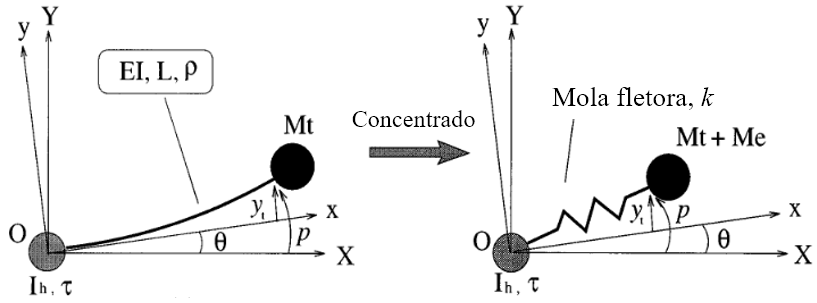
\includegraphics[width=0.75\textwidth]{figs/lumped}
 	\caption[Modelo de parâmetros concentrados]{Modelo de parâmetros concentrados
 	\\ Fonte: adaptado de \cite{zhu1999simulation}}
 	\label{fig::lumped}
\end{figure}

Realizando o desenvolvimento pelas equações de Lagrange, obtém-se as equações de
movimento deste sistema na forma:
%
\begin{gather}
	M \ddot{p} = -k(p-L \theta) \\
	I_h \ddot{\theta} - k L(p-L \theta) = \tau
\end{gather}
%
Onde $\tau$ representa o torque de acionamento do braço, na direção $Z$.

Este método, apesar de ser orientado para manipuladores com flexibilidade em
seus elos, mostra-se interessante para modelar a base flexível do manipulador.
Fazendo-se as devidas adaptações, pode-se considerar a base como um dos elos
flexíveis do robô e obter-se a rigidez e inércia de sua estrutura, e chegar-se
às equações de movimento de modo equivalente.


\subsection{Manipuladores sobre bases flexíveis}

Em sistemas de manipuladores sobre bases móveis, o acoplamento dinâmico entre o
braço robótico e sua base prejudica a acurácia de posicionamento e a destreza
operacional do robô. \citet{yoshida1996moving} classificam estes sistemas em
quatro categorias:
%
\begin{enumerate*}[label=\alph*)]
	\item manipulador de flutuação livre;
	\item manipulador montado sobre estrutura flexível;
	\item macro-micro manipuladores;
	\item manipulador montado sobre veículo móvel.
\end{enumerate*}
%
É interessante notar que a metodologia desta pesquisa permite analisar qualquer
um destes sistemas, embora os estudos de caso tenham se focado em bases que se
enquadram no o item \emph{b} da classificação. A Figura~\ref{fig::classes_bases}
ilustra cada classe esquematicamente.

\begin{figure}[h]
	\centering 
 	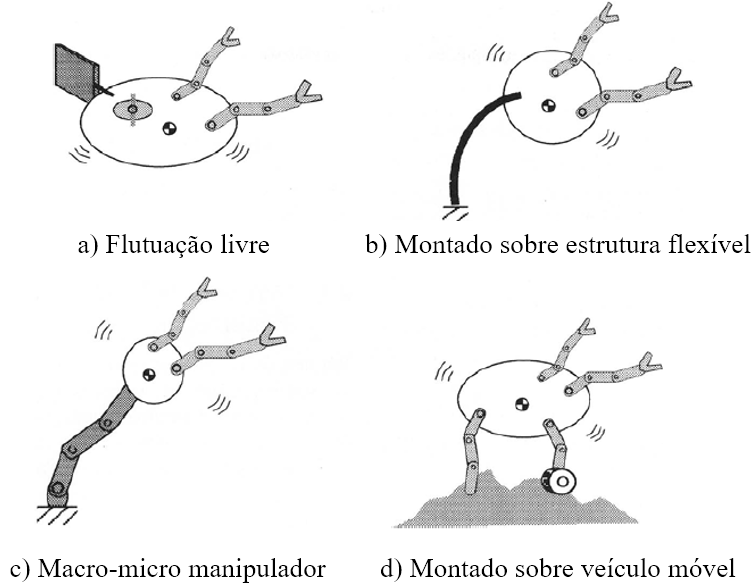
\includegraphics[width=0.75\textwidth]{figs/classes_bases}
 	\caption[Classes de manipuladores sobre bases móveis]{Classes de
 	manipuladores sobre bases móveis \\ Fonte: adaptado de
 	\cite{yoshida1996moving}}
 	\label{fig::classes_bases}
\end{figure}

Como exemplo de manipuladores em flutuação livre são os robôs de serviço
espaciais, dedicados à manutenção de sistemas em órbita, o que inclui
o reparo, montagem, reabastecimento e melhorias em espaçonaves, após
implantação~\cite{flores2014review}. Este sistema é apresentado na
Figura~\ref{fig::space_robot}, em que um sistema com robô captura uma
espaçonave  para realizar um seriço em órbita.

\begin{figure}[h]
	\centering 
 	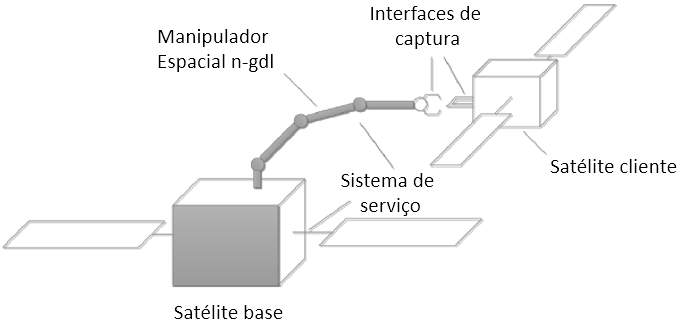
\includegraphics[width=0.75\textwidth]{figs/space_robot}
 	\caption[Manipulador sobre base flutuante em órbita]{Manipulador sobre base
 	flutuante para operação em órbita. \\ Fonte: adaptado de
 	\cite{flores2014review}}
 	\label{fig::space_robot}
\end{figure}

Os macro-micro manipuladores são sistemas robóticos em que é necessário longo
alcance, ao mesmo tempo que realiza tarefas de precisão em seu
efetuador~\cite{sharon1993macro}.
Isto é feito pelo uso de dois manipuladores em série, em que o primeiro (macro)
tem o objetivo de posicionamento e alcance elevado, com uso de braços compridos
e esbeltos, o que os torna bastante flexíveis; e o segundo (micro), realiza a
tarefa num espaço de trabalho reduzido e equipado com a ferramenta para
operação, como pode ser verificado na Figura~\ref{fig::macro_micro}. Nesta
classe de sistemas, o macro-manipulador pode possui flexibilidade tanto nos elos
quanto nas juntas e o micro-manipulador é considerado rígido.
Diversos métodos de controle foram propostos como a estabilização do sistema
pelo controle apenas do micro-manipulador~\cite{book1989vibration} ou controle
do planejamento de trajetória para minimizar as vibrações~\cite{torres1993path},
que apresenta uma técnica chamada Mapa de Acoplamento (ou \textit{Coupling
Map}). 

\begin{figure}[h]
	\centering 
 	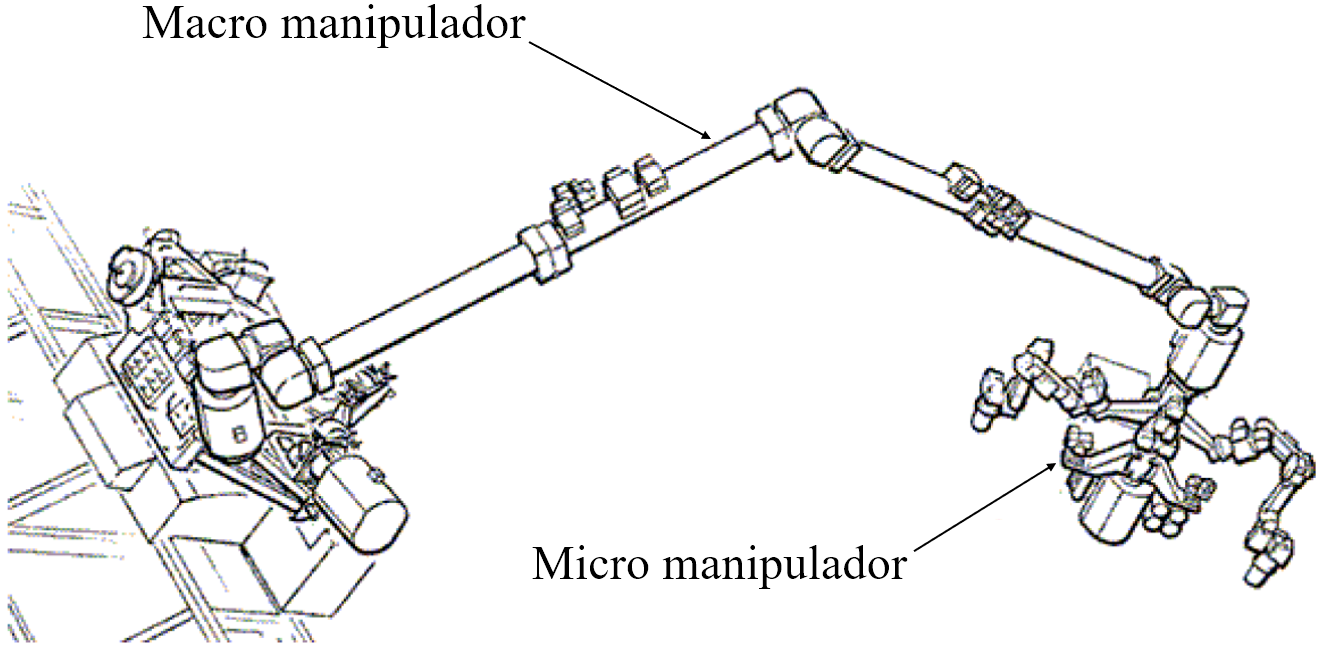
\includegraphics[width=0.70\textwidth]{figs/macro_micro}
 	\caption[Macro-micro manipulador]{Macro-micro manipulador para satélite \\
 	Fonte: adaptado de \cite{schubert2000impedance}}
 	\label{fig::macro_micro}
\end{figure}

Os manipuladores montados sobre estruturas flexíveis podem ser tratados como
casos especiais de sistemas macro-micro manipuladores. Nestes casos, a base na
qual o robô está fixado é excitada pelo movimento do braço robótico e aparecem
grandes deslocamentos devido à elasticidade da estrutura da base.
Geralmente, os métodos de controle destes sistemas associam-se a duas classes:
controle do amortecimento~\cite{george2002inertial}, \cite{lew2001simple} e
controle do ponto final do efetuador~\cite{sharon1993macro},
\cite{torres1993path}. No controle de ponto final, a posição e orientação
precisam ser medidas com respeito a um referencial inercial, podendo ser medidos
indiretamente como por exemplo, com extensômetros no ponto de acoplamento da
estrutura com o robô~\cite{mavroidis1997optimal}.
A vantagem deste método é que não é necessário interromper a tarefa para
amortecer as vibrações da estrutura de suporte. O sistema Shaky II apresentado
na Figura~\ref{fig::shaky} foi desenvolvido~\cite{mavroidis1997optimal}
para avaliar a dinâmica desta classe de sistema robótico e validar
experimentalmente métodos de controle por controle de ponto final inferido.

\begin{figure}[h]
	\centering 
 	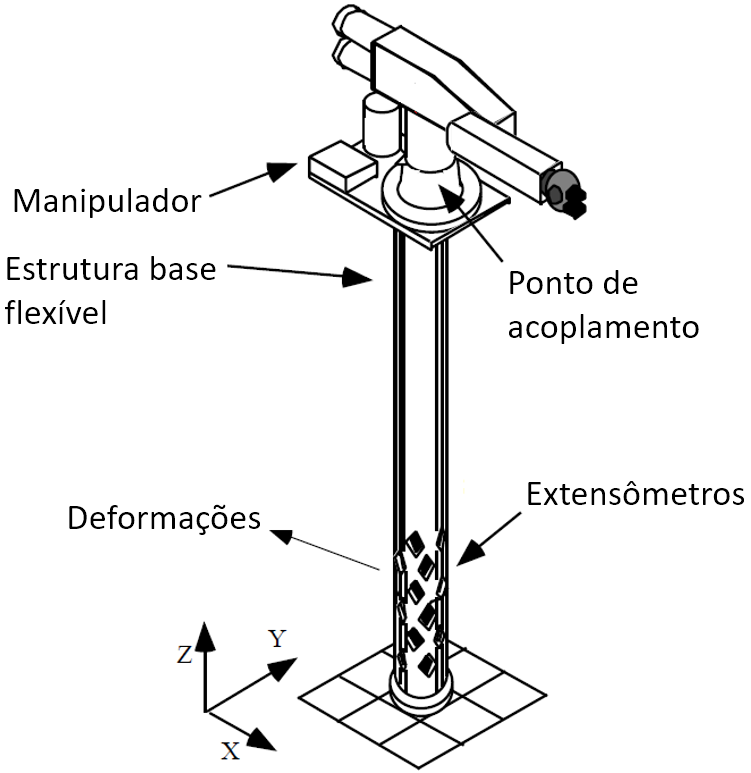
\includegraphics[width=0.50\textwidth]{figs/shaky}
 	\caption[Estrutura experimental do Shaky II]{Estrutura experimental do Shaky II para validação de
 	controle de ponto final. Fonte: adaptado de \cite{mavroidis1997optimal}}
 	\label{fig::shaky}
\end{figure}

Outra solução para evitar vibrações e grandes amplitudes de deformação é o
de escoramento ou contravetamento dos elementos flexíveis no
ambiente~\cite{lew1994bracing}. O escoramento em estruturas estacionárias
ajudaria a enrijecer e amortecer a estrutura flexível e evitar grandes erros de
posicionamento do efetuador. Esta estratégia é explorada nesta pesquisa no
sentido de verificar configurações de base que satisfazem a rigidez necessária para o
processo.

Seja o vetor de coordenadas generalizadas representado por $\boldsymbol{\xi} =
[\phi, q]$, onde $\boldsymbol{\phi} = [x, y, z, \theta_x, \theta_y, \theta_z]$
são as coordenadas generalaizadas da base, o sistema dinâmico do manipulador sobre base móvel pode
ser expresso por:
%
\begin{equation}
	H(\xi) \ddot{\boldsymbol{\xi}} + C(\xi , \dot{\xi}) \dot{\boldsymbol{\xi}} + K
	\boldsymbol{\xi} = \boldsymbol{\Xi}
\end{equation}
%
Onde $H(\xi) \in \Re^{6+n \times 6+n}$ é a matriz de inércia acoplada, $C$ e $K
\in \Re^{6+n \times 6+n}$ contém em $C$ os termos de amortecimento viscoso da
base e centrífugos e de Coriolis do braço robótico, e em $K$ a matriz de rigidez
da base.
O vetor $\boldsymbol{\Xi} = [0, \tau]$ contém os torques externos de controle do
manipulador e considera as forças externas na base nulas. Na forma matricial,
pode-se escrever a matriz de inércia acoplada como:
%
\begin{equation}
	H(\xi) = \begin{pmatrix}
			H_b 	&	H_{bm} \\ 
			H_{bm}	&	H_m
\end{pmatrix}
\end{equation}
%
Em que o termo $H_b \in \Re^{6}$ representa o tensor de inércia da base, $H_m
\in \Re^{n}$ representa o tensor de inércia do manipulador, onde $n$ é o número
de graus de liberdade, e $H_{bm}$ o tensor de inércia do acoplamento
base-manipulador.

Será interessante notar que estes termos de acoplamento serão calculados
automaticamente ao seguir o procedimento sistemático das rotinas do Sophia,
sendo necessário apenas fornecer as matrizes $H_b$ e $H_m$ isoladamente assim
como a cadeia de sistemas de referência locais para se chegar ao modelo
acoplado. No método proposto, a interação entre base e robô, que gera forças devido a
rigidez e amortecimento da base, e são tratados como esforços externos
proporcionais ao deslocamento e velocidade do ponto de acoplamento. E os termos
de Coriolis e centrífugos também surgem do cálculo algébrico com as
funções do Sophia, sem a necessidade de investigar estes termos individualmente. 



\subsection{Tarefas robóticas \textit{in situ}} \label{sec::insitu}

Hoje os robôs não estão mais limitados a operações de fábrica e estão
substituindo atividades humanas fora do ambiente industrial, seja por segurança,
eficácia ou produtividade. Operações robóticas de inspeção ou manutenção de
equipamentos realizadas no próprio local onde operam, ou \textit{in situ}, são
perigosas ou de difícil acesso para realização humana. Por isso, soluções
utilizando robôs para executar tais tarefas têm se tornado uma alternativa
atraente . Os manipuladores da classe macro-micro são uma solução interessante
para essas operações porque fornecem um espaço de trabalho ampliado pelo
manipulador macro, assim como toda a precisão e agilidade de um manipulador
micro.

\begin{figure}[h]
	\centering 
 	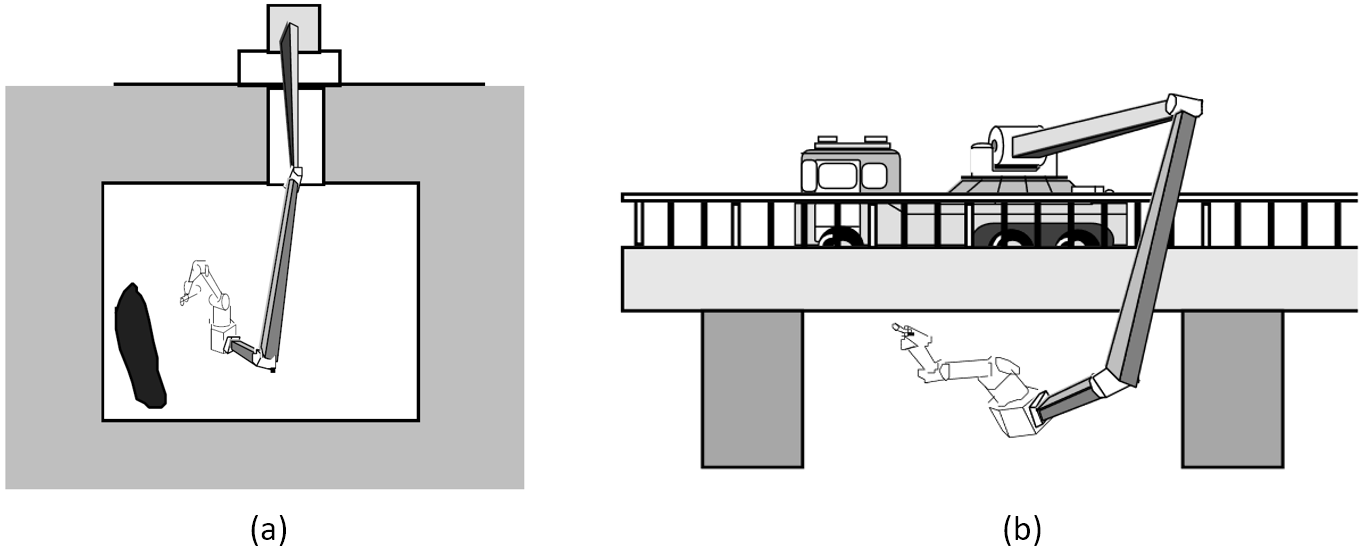
\includegraphics[width=0.95\textwidth]{figs/inspection_robots}
 	\caption[Robôs de inspeção \textit{in situ}]{Robôs de inspeção \textit{in
 	situ}: a) tanques subterrâneos; b) pontes. \\ Fonte: adaptado de \cite{mavroidis1995end}}
 	\label{fig::inspection_robots}
\end{figure}

Um exemplo desta classe de robôs de serviço é o sistema de remoção e transporte
de resíduos nucleares (WD\&C) de tanques subterrâneos, cujo acesso é limitado
(Figura~\ref{fig::inspection_robots}a). Um manipulador longo e esbelto permite
a entrada pelo duto de acesso e o posicionamento do robô menor para alcançar e
remover o material do tanque~\cite{knape1990development}. Outro exemplo é de
sistema robótico de longo alcance para inspeção de pontes
(Figura~\ref{fig::inspection_robots}b). Para sistemas como esse em que a
inspeção é feita por imagens~\cite{oh2009bridge}, as vibrações da ponte
propagadas pelos elos do manipulador, e condições de vento por exemplo, podem
tornar as imagens borradas e inutilizáveis.

Uma lista crescente de serviços \textit{in situ} já podem ser realizados por
robôs como por exemplo: pintura, limpeza, manutenção, cirurgias, montagem de
veículos espaciais, armamento militar, agricultura e
outros~\cite{nof1999handbook}. Em todos estes casos, onde o ambiente não é
normalmente preparado para a tarefa, que na maioria das vezes é apenas
temporária, e por isso há que se prever o comportamento dinâmico do sistema
robô-base-ambiente para que se garanta a qualidade da tarefa.


\subsubsection{EMMA - Protótipo para revestimento de turbinas
hidráulicas \textit{in situ}}

As turbinas hidráulicas de geração de energia do tipo Kaplan sofrem danos em
suas pás devido, principalmente, a efeitos de abrasão e cavitação relativo aos
escoamento.
Antes de serem instaladas, estas pás recebem um revestimento metálico de carbeto
de tungstênio, que protege contra os efeitos do escoamento. Com o tempo esta
proteção se desgasta e inicia um processo de degradação da pá, causando
vibrações, instabilidade do escoamento e perda de eficiência
energética~\cite{escaler2006detection}.

\begin{figure}[h]
	\centering 
 	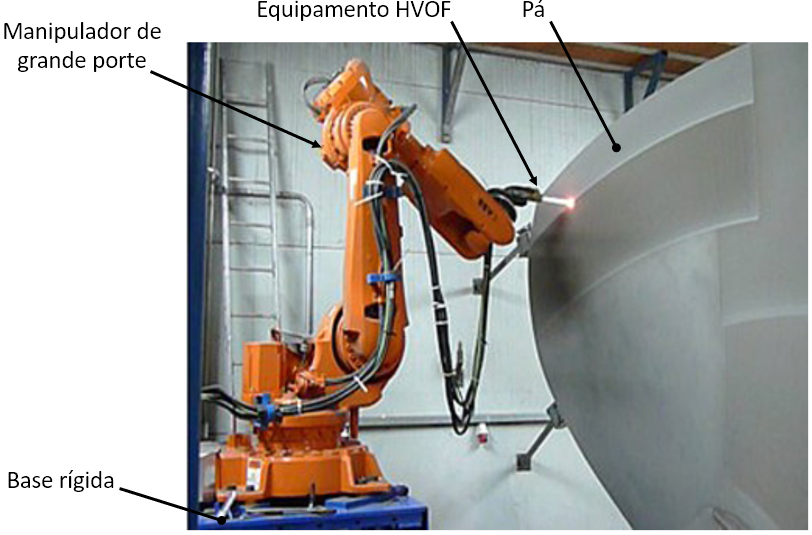
\includegraphics[width=0.80\textwidth]{figs/rijeza_hvof}
 	\caption[Aplicação de revestimento em ambiente industrial]{Aplicação de
 	revestimento em ambiente estruturado.
 	Fonte: adaptado de website da Rijeza, disponível em www.rijeza.com.br
 	(acessado em Mar-2018)}
 	\label{fig::rijeza_hvof}
\end{figure}

Para evitar este problema, o revestimento deve ser reaplicado em períodos
programados de manutenção. Isto implica, hoje, em parar a unidade geradora,
desmontar as pás, levar até a área de manutenção e reaplicar o revestimento fora
do ambiente da turbina, resultando em um procedimento de alta complexidade
operacional de manobra e transporte, riscos, alto custo e principalmente: tempo
de parada de máquina. A Figura~\ref{fig::rijeza_hvof}
apresenta o revestimento sendo aplicado antes da instalação por um braço
robótico, em ambiente industrial e bem estruturado.

Como uma alternativa para manutenção das pás, foi projetado um sistema robótico,
denominado EMMA, para reaplicação do revestimento dentro da unidade geradora,
que dispensa a necessidade de desmontagem das pás, realizando todo o processo de
aplicação \textit{in situ}. Este sistema tem o desafio de lidar com o difícil
e limitado acesso, operar em ambiente confinado, de superfície curva, inclinada
e escorregadia, alta umidade e temperatura. Pelo acesso ser limitado a uma
escotilha de $800~mm$ e outra de $350~mm$ de diâmetro, o sistema deve ser
modular e leve, a fim de ser transportado e montado manualmente no interior da
turbina. A Figura~\ref{fig::turbina_ug} ilustra o interior da unidade geradora,
destacando os principais equipamentos no interior e indicando os acessos da
escotilha superior e escotilha inferior.

\begin{figure}[h]
	\centering 
 	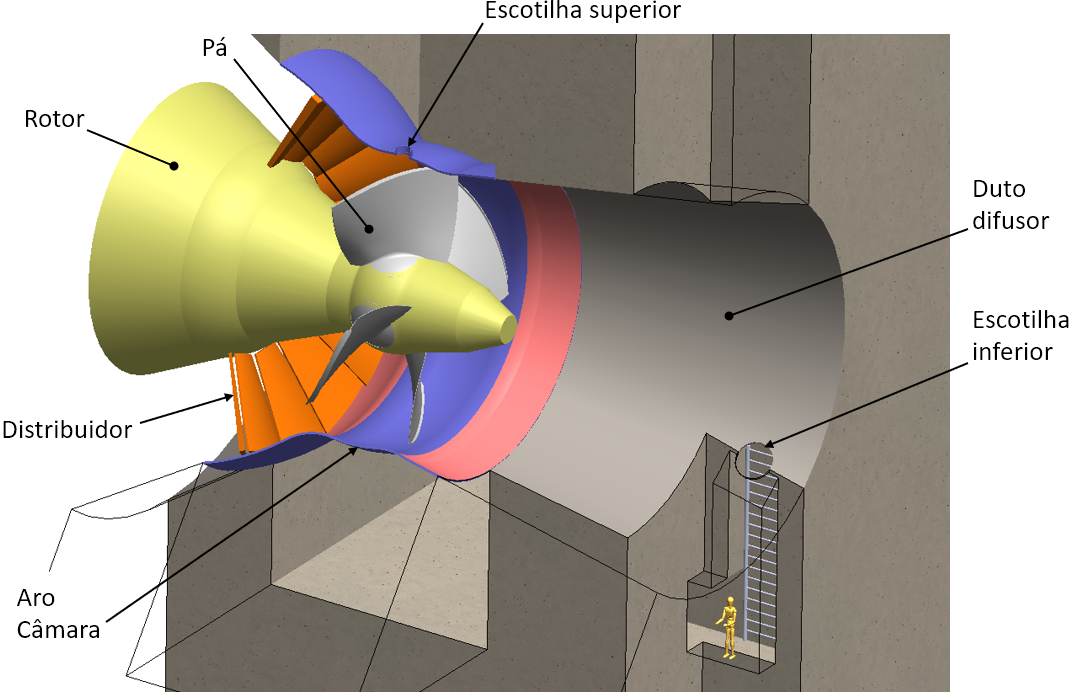
\includegraphics[width=0.90\textwidth]{figs/turbina_ug}
 	\caption{Vista esquemática do interior da unidade geradora}
 	\label{fig::turbina_ug}
\end{figure}

Outro desafio é atender aos requisitos do processo de revestimento. A técnica
utilizada de revestimento por asperção térmica chamada HVOF (de \textit{high
velocity oxy-fuel}) requer o aparato apresentado na
Figura~\ref{fig::hvof_aparato}. Neste processo, uma mistura de combustível e
oxigênio é alimentadando continuamente a uma câmara de combustão. O gás
resultante emana do bocal em um jato, a uma velocidade normalmente acima de
$1000~m/s$, onde as partículas de carbeto de tungstênio se misturam, se
aquecendo, acelerando e colidindo contra o material base, formando a camada de
revestimento~\cite{kuroda2008warm}.

\begin{figure}[h]
	\centering 
 	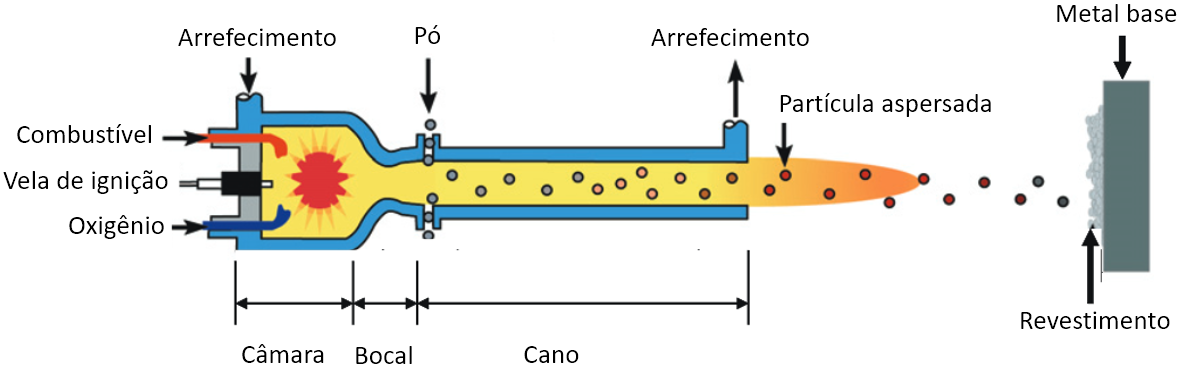
\includegraphics[width=0.90\textwidth]{figs/hvof_aparato}
 	\caption[Aparato do processo de revestimento por HVOF]{Aparato do processo de
 	revestimento por HVOF. \\ Fonte: adaptado de~\cite{kuroda2008warm}}
 	\label{fig::hvof_aparato}
\end{figure}

Para obter uma camada regular de revestimento, é necessário obedecer requisitos
de velocidade da pistola, distância para o metal base, orientação e passo. A
Tabela~\ref{tab::req_hvof} resume os principais dados do processo HVOF.

\begin{table}[h]
\centering
\caption[Dados do processo HVOF para revestimento da pá]{Dados do processo HVOF
para revestimento da pá. Fonte: \citet{freitas2017state}}
\label{tab::req_hvof}
\begin{tabular}{@{}ll@{}}
\toprule
\textbf{Componente}           							& \textbf{Valor}  		\\ \midrule
Massa da pistola HVOF        							& 8 kg           		\\
Temperatura da chama         							& 3000$^{\circ}$ C  	\\
Empuxo da pistola             							& 15 N           		\\
Passo entre parelelos da trajetória	   	    			& 3 mm  				\\
Distância da pistola para a pá 							& 230-240 mm 			\\
Ângulo da pistola para a superfície da pá				& 90$^{\circ}$      	\\
Velocidade perpendicular à superfície da pá  			& 40 m min$^{-1}$   	\\
Ruído sonoro do HVOF          							& 100-140 dB    		\\
Temperatura da pá              							& até 110$^{\circ}$ C 	\\ \bottomrule
\end{tabular}
\end{table}

Nota-se pelos dados apresentados a impossibilidade de se realizar esta tarefa
manualmente e a necessidade de ter um sistema preciso para realizá-la por robô,
a fim de atender aos requisitos do processo.

Pela limitação de acesso e espaço apertado próximo às pás, um dos principais
critérios para seleção do manipulador foi seu tamanho. Isto implica em um
espaço de trabalho reduzido em relação ao tamanho da pá, o que resulta na
necessidade de fixar o robô em mais de uma posição a fim de cobrir
toda a face. Para isso é necessária uma base com graus de liberdade suficientes,
que permitam a mudança de posicionamento do robô, para cada região da pá. 

O projeto EMMA estudou diversos conceitos de base, que foram classificados de
acordo com os graus de liberdade fornecidos. Dentre eles, destacam-se os
conceitos Prismático-Rotacional-Prismático-Prismático (PRPP), da
Figura~\ref{fig::base_telesc_turbina} e Prismático-Rotacional-Prismático (PRP),
da Figura~\ref{fig::prp_turbina}. Note-se que estes conceitos de base podem ser
modelados exatamente como o sistema macro-micro manipulador, a base (macro) para
posicionamento, ignorando-se a atuação das juntas do sistema macro, e o braço
robótico (micro) para realizar a tarefa, como é exposto em
\cite{sharon1993macro} e \cite{lew1994bracing}.

O sistema de base PRPP consite em um mecanismo telescópico com atuadores
lineares para os braços prismáticos e uma junta rotacional. A estrutura é fixada
na entrada da escotilha de acesso superior da unidade geradora e o robô é fixado
na extremidade do último braço da estrutura telescópica. Isto permite que o
manipulador seja posicionado diversas vezes para cobrir toda a face da pá. No
entanto, o dimensionamento estrutural verificou que apesar de a estrutura
suportar com boa margem as tensões a que seria submetida, os deslocamentos
devido à baixa rigidez poderiam reduzir a precisão do robô em realizar a tarefa
de revestimento.

\begin{figure}[t]
	\centering 
 	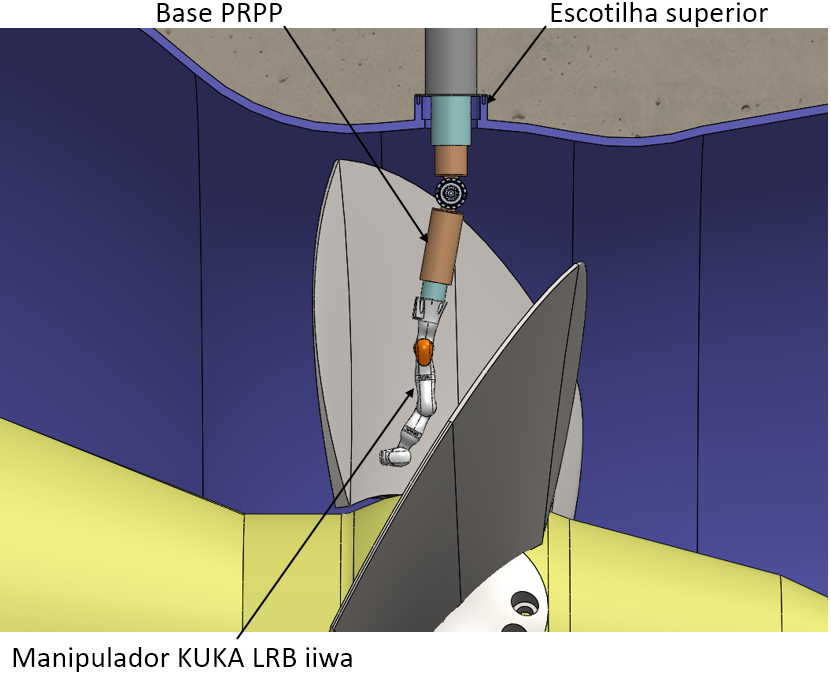
\includegraphics[width=0.65\textwidth]{figs/base_telesc_turbina}
 	\caption{Base telescópica PRPP para manutenção de revestimento
 	\textit{in-situ}}
 	\label{fig::base_telesc_turbina}
\end{figure}

\begin{figure}[h]
	\centering 
 	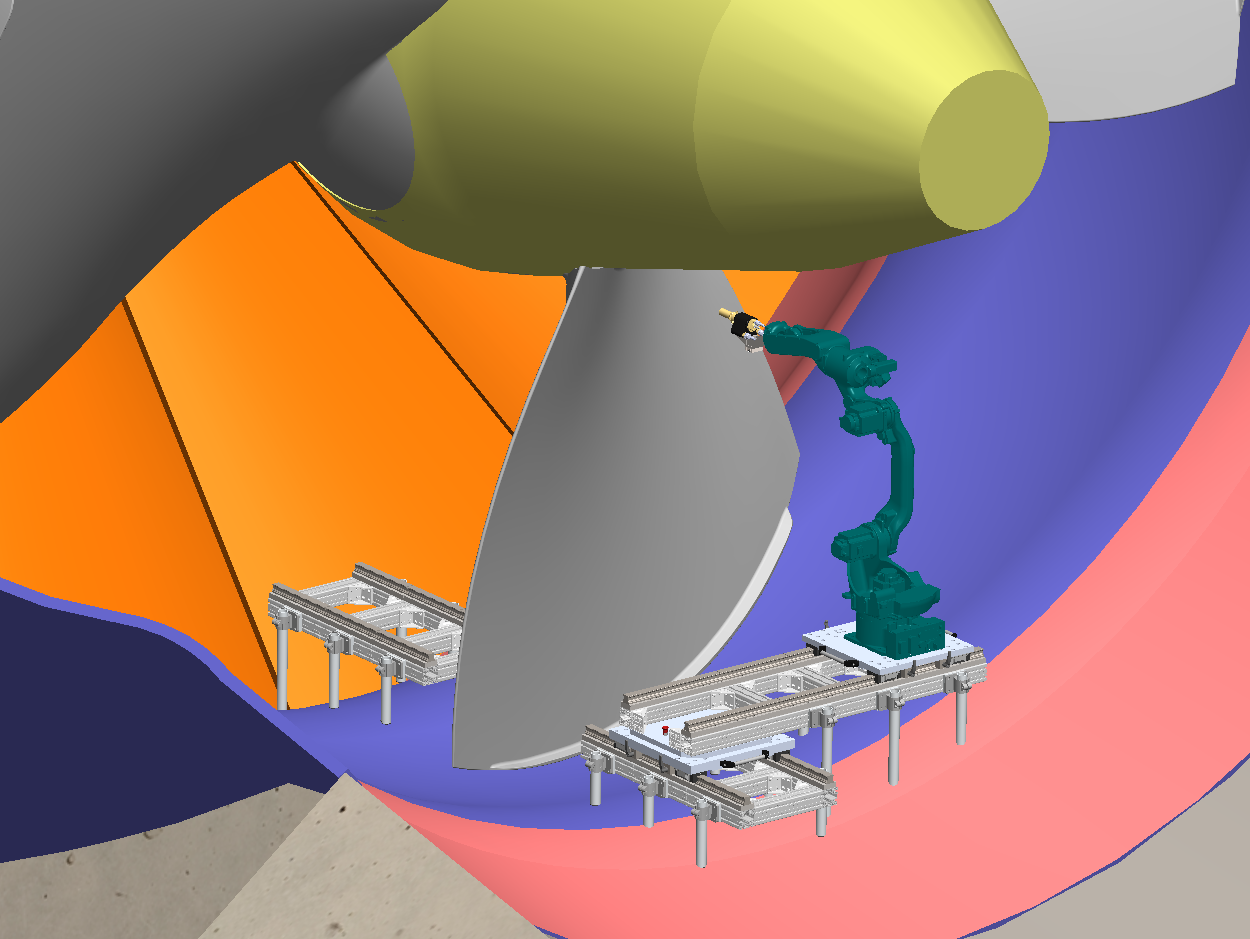
\includegraphics[width=0.70\textwidth]{figs/prp_turbina}
 	\caption{Base modular PRP para manutenção de revestimento \textit{in-situ}}
 	\label{fig::prp_turbina}
\end{figure}

O conceito PRP utiliza o acesso da escotilha inferior para transportar uma base
modular para o interior da unidade geradora. Esta base é composta por uma
estrutura de alumínio equipada com trilhos paralelos, que concedem ao sistema o
movimento linear ao longo da esturutra. Uma plataforma de rotação funciona como
uma junta entre os trilhos, o que permite que estes formem qualquer ângulo entre
si e fornecendo 3 graus de liberdade à base. Pela limitação do acesso, a
estrutura da base deve ser modular e leve, porque sofrerá diversas montagens,
desmontagens e transportes manuais.Como resultado, obtém-se uma estrutura leve e
versátil, mas não superdimensionada para rigidez. De toda forma, uma vantagem
deste conceito encontra-se na possibilidade adicionar suportes e
contraventamentos à estrutura, o que permite aumentar a sua rigidez.

A presente pesquisa trata estes conceitos e a tarefa de revestimento do projeto
EMMA como os estudos de caso para demonstração da aplicação do método proposto,
que consiste em quantificar os erros causados pelos deslocamentos elásticos da
base e investigar se são toleráveis ou não para garantir a qualidade da tarefa.


















